\documentclass{article}
\usepackage{graphicx}
\usepackage{times}
\usepackage{graphicx}
\usepackage{hyperref}
\usepackage{enumitem}
\usepackage{longtable}
\usepackage{booktabs}
\usepackage{array}
\usepackage{ragged2e}
\usepackage{pgfgantt}
\usepackage{amssymb}
\usepackage{amsmath}
\usepackage{pdflscape}
\usepackage[
backend=biber,
]{biblatex}
\usepackage{titlesec}

\newcommand{\subsubsubsection}[1]{\paragraph{#1}\mbox{}\\}
\setcounter{secnumdepth}{4}
\setcounter{tocdepth}{4}

\addbibresource{Bibliography.bib}

\title{Pre-runtime Structural Analysis for Quantum Software Quality}
\author{Cristian Marquez, }
\author{It's me\\[1cm]{\small Advisor: A.D.Visor}}

\author{
  Marquez, Cristian\\
  \texttt{c.marquezb@uniandes.edu.co}
  \and
  Advisor: Kelly, Garces\\
  \textit{Universidad de los Andes}\\
  Bogotá, Colombia \\
  \texttt{kj.garces971@uniandes.edu.co}
  \and
  Co-Advisor: Sierra, Daniel\\
  \textit{The Catholic University of America}\\
  Washington DC, 20064 \\
  \texttt{sierrasosa@cua.edu}
}

\date{March 2026}

\begin{document}

\begin{titlepage}
    \centering
    
    % University logo
    \includegraphics[width=0.25\textwidth]{logo_uniandes.png}\\[1cm]
    
    {\Large \textbf{Universidad de los Andes}}\\[0.3cm]
    {\large Facultad de Ingeniería}\\[0.3cm]
    {\large Departamento de Ingeniería de Sistemas y Computación}\\[1.5cm]
    
    {\large \textbf{Thesis Proposal}}\\[1.5cm]
    
    {\LARGE \textbf{Pre-runtime Structural Analysis for Quantum Software Quality}}\\[1cm]
    
    {\large \textbf{Student}}\\
    Cristian Marquez\\
    \textit{Universidad de los Andes}\\
    Bogotá, Colombia \\
    \texttt{c.marquezb@uniandes.edu.co}\\[1.5cm]
    
    {\large \textbf{Advisor}}\\
    Kelly Garces\\
    \textit{Universidad de los Andes}\\
    Bogotá, Colombia \\
    \texttt{kj.garces971@uniandes.edu.co}\\[1cm]
    
    {\large \textbf{Co-Advisor}}\\
    Daniel Sierra-Sosa\\
    \textit{The Catholic University of America}\\
    Washington DC, 20064 \\
    \texttt{sierrasosa@cua.edu}\\[2cm]
    
    \vfill
    
    {\large Bogotá, Colombia}\\
    {\large March 2026}
    
\end{titlepage}

\section{Abstract}

This research addresses key challenges in quantum computing (QC) by proposing a quality model for quantum software grounded in the principles of software measurement theory. Given the inherent limitations of today's noisy intermediate-scale quantum (NISQ) hardware, there is a lack of metrics and tools necessary to evaluate key quality metrics (e.g. fidelity and success rate) of a quantum circuit before committing it to execution. This thesis addresses this research gap by formally defining, empirically validating, and implementing a set of quality metrics as part of a predictive model.

To address these challenges systematically, the foundation for this research was established through three interconnected studies. First, a systematic mapping review confirmed the early stage of QC and highlighted a research opportunity to develop quality metrics for the quantum domain. Second, an analysis of quantum development tools revealed a gap between theoretical metrics and practical implementation, motivating the creation of qWard, a Python library designed to analyze quantum circuits. Finally, an experiment utilizing the teleportation protocol demonstrated a quantifiable link between a circuit's structural characteristics and its execution reliability on real hardware. Together, these studies have produced two open datasets comprising 1{,}573 real QPU executions on IBM and Rigetti hardware, which serve as the empirical foundation for the predictive framework proposed in this thesis.

Building on these foundations, the central contribution of this thesis is the Quality-Aware Quantum Software (QAQS) framework, a pre-runtime quality model for quantum software. QAQS introduces a temporal classification that distinguishes between pre-runtime metrics, derived from static analysis of the circuit representation, and post-runtime metrics, obtained from execution results. At its core, QAQS defines the "circuit footprint," a curated feature vector of pre-runtime metrics that captures the essential characteristics of a quantum circuit, condensing a complex artifact into a compact representation for quality analysis.

To validate the practical utility of the footprint, classical supervised regression models are trained to predict post-runtime quality metrics from pre-runtime features. As a secondary, boundary-setting analysis, the study compares the circuit-only footprint (i.e., the transpiled-circuit features without explicit backend calibration) against two hardware-aware variants, one using calibration data only and one combining both sources, to characterize whether explicit hardware context is necessary for cross-provider prediction. The framework is evaluated across six algorithms organized into three paradigms, i.e., groups of algorithms that share the same core quantum mechanism. \emph{(i)} The Fourier-based paradigm includes the Quantum Fourier Transform (QFT) and Phase Estimation (PE); \emph{(ii)} the oracle-based paradigm includes Grover's search (GO) and Bernstein-Vazirani (BV); and \emph{(iii)} the entanglement-based paradigm includes the variation of the Teleportation Protocol (vTP) and the preparation of GHZ states. All algorithms will be executed on quantum computing backends provided by IBM and Rigetti, with IonQ resources utilized conditional upon availability of access.

Notice that the algorithm selection is restricted to those where the expected output quantum states are known a priori, thereby allowing the Differential Success Rate (DSR) to be employed as a complementary fidelity metric together with measures like Hellinger fidelity (HF) and Total Variation Distance (TVD). In contrast, paradigms such as the Variational Quantum Eigensolver (VQE) or Hamiltonian simulations are excluded because their outputs lack a discrete set of dominant states, requiring instead an analysis of the full probability distribution that falls outside the scope of this work.

Ultimately, this research contributes to the emerging discipline of quantum software quality engineering through QAQS, which integrates the circuit "footprint" as its empirically grounded feature vector, an open-source measurement toolkit (qWard), a distribution-aware post-runtime metric (DSR), and a predictive model that validates the "footprint" using real QPU executions. By establishing a data-driven link between a circuit's structure and its real-world performance, QAQS aims to make quantum software development more transparent and predictable, contributing to the path toward practical quantum advantage.

\newpage

\tableofcontents

\newpage

\section{Introduction}
\label{section:introduction}

QC is an emerging field based on the principles of quantum mechanics \cite{Maslov2019} that enables systems to take advantage of phenomena such as superposition and entanglement to address computational challenges that are infeasible for classical systems. This novel approach has the potential to improve the way humans solve complex problems such as large-scale number factorization \cite{Willsch2023}, cryptography \cite{Upadhyay2019}, model training \cite{Biamonte2017, AdvancesinQuantumDeepLearning}, and any problem that requires high computational resources.

This transformative potential of QC has garnered considerable attention, leading to substantial investment and generating significant momentum within the field, as documented by Gartner and McKinsey reports \cite{McKinsey}. Recent technological advances, coupled with increased funding, have further propelled this momentum. That said, QC is still in its nascent stages, with significant challenges to overcome before it can be widely adopted, particularly in integrating quantum capabilities into classical computing environments, a critical step for realizing its full potential.

This early stage of development is clearly reflected in the quantum software ecosystem. During the past decade, quantum software engineers have developed domain-specific programming languages such as Quantum Computation Language (QCL) \cite{OmerQCLProgramming} and Q\# \cite{MicrosoftQ}, alongside software development kits (SDK) such as Azure Quantum \cite{Bradben2024AzureQuantum}, Ocean SDK \cite{DwaveOceanSdk2024} and Qiskit \cite{IBMQiskit2024}. Although these tools represent significant progress, the use of quantum algorithms to solve real problems is still in its infancy \cite{Ruefenacht2022}. Recent efforts, such as the creation of an enterprise service bus to connect classical and quantum systems \cite{Bonilla2024}, highlight the ongoing push to integrate QC into existing pipelines.

Despite the availability of these development tools, the high economic cost, the noisy hardware, and uncertainty associated with the execution of quantum circuits remain critical challenges. As QPUs become more accessible, the community's focus has shifted from the feasibility of hardware construction to the reliability of execution. However, the cost of quantum runtime services is substantial\footnote{For example, as of 2025, major providers charge significant rates per second or per shot for on-demand QPU access, making iterative testing prohibitively expensive.} compared to classical resource prices. This economic reality emphasizes the need for robust methodologies that can analyze and forecast quantum circuit behavior prior to execution.

To ensure reliable results, developers currently rely on a combination of logical qubits and general benchmarking protocols, yet these approaches have significant limitations for predictive analysis. Logical qubit abstraction aims to mitigate errors, but its hardware-dependent implementation makes it difficult for a developer to anticipate how a unique circuit structure will interact with the error correction layer. Similarly, hardware-centric benchmarks like Quantum Volume \cite{proctorBenchmarkingQuantumComputers2025_2025} provide a single holistic score based on random circuits, which reveals little about how a specific user-defined algorithm will behave. This failure to deliver circuit-specific predictive insights makes these existing approaches unsuitable to improve the understandability of custom circuits or to serve as a foundation for reliability models.

This disconnect has created an opportunity for research in the field of application oriented benchmarking that can bridge the gap between general hardware capability and specific circuit reliability \cite{millsApplicationMotivatedHolistic2021}. Addressing this gap requires moving beyond purely hardware-focused evaluations to a metric-based approach. Specifically, this thesis proposes a temporal classification that organizes quantum circuit metrics into a quality model for quantum software. As the quantum development lifecycle involves two distinct phases--- circuit creation and execution---a temporal classification naturally separates metrics into \textbf{pre-runtime metrics}, such as circuit depth and gate count, which can be computed after coding but before execution, and \textbf{post-runtime metrics}, such as success rates and fidelity, which are derived from the execution itself.

Building upon this temporal classification, this thesis defines the circuit "footprint," a curated feature vector of pre-runtime metrics that characterizes the quality of a quantum circuit. The research validates this quality model by demonstrating that the footprint has sufficient predictive power to estimate post-runtime outcomes such as DSR, HF, and TVD. To delineate the boundaries of this pre-runtime approach, the study also compares the circuit-only footprint, which besides the implicit structural encoding produced by transpilation does not incorporate explicit backend calibration data, against two hardware-aware variants (calibration-only and a mixed configuration that combines circuit and calibration features), assessing whether explicit backend context is required for cross-provider prediction. This quality model, named Quality-Aware Quantum Software (QAQS), encapsulates the circuit footprint, its measurement toolkit, and its validation pipeline, aiming to evaluate the expected quality of quantum algorithms before execution and thereby transforming quantum development from a costly trial-and-error process into a more predictable engineering discipline.

The rest of the document is structured as follows. Section~\ref{section:background} presents the background, establishing the algorithmic paradigms, the metric taxonomy, and the quality concepts that form the basis of this research. Section~\ref{section:related-work} reviews related work on quantum circuit prediction. Section~\ref{section:problem-statement} formulates the problem statement, research question, hypotheses, and objectives. Section~\ref{section:methodology} outlines the research methodology. Section~\ref{section:qaqs} introduces the QAQS proposal. Section~\ref{subsec:scope} defines the scope and delimitations. Section~\ref{section:contributions} describes the expected contributions. Finally, Section~\ref{section:work} presents the research plan and timeline.

\section{Background}
\label{section:background}

This section provides the foundations for the predictive framework developed in this thesis. It first describes the typical workflow of a quantum application and the algorithmic paradigms considered in this research. It then details the taxonomy adopted to categorize quantum circuit metrics, and concludes with a discussion of related work.

\subsection{The Quantum Algorithm Workflow}
\label{subsec:qc-workflow}

The deterministic nature inherent in classical computing enables a development workflow in which developers remain unquestioning of their results. In contrast, quantum phenomena are stochastic, which prevents developers from trusting their results after a single execution. As a result, QC output is typically represented as histograms, leading to the emergence of a novel development paradigm. This new paradigm focuses on formulating QC algorithms that target the probability distribution of an outcome instead of a fixed value.

To address this challenge, runtime quantum services introduce three distinct concepts. The first concept, termed \textbf{Job}, refers to a singular invocation of the quantum service. Within the context of a \textbf{Job}, the developer specifies the number of \textbf{Shots}, which indicates the number of times an algorithm is executed within a single service request. Moreover, if necessary, developers have the option to execute multiple \textbf{Jobs} in \textbf{Batches}, which is an available approach to explore different configurations of the runtime service, including adjustments to circuit optimizations, variations in the initial qubits layout, or changes in routing strategy.

This execution model reflects a fundamental difference regarding how program correctness is verified. In classical computing, successful execution is validated by directly comparing the observed output against an expected value since each execution produces a reproducible result. In contrast, in the quantum realm, a single run of an algorithm produces only a single classical state \cite{nielsenQuantumComputationQuantuma_2010}, and the developer must construct a probability distribution over all possible outcomes by accumulating many shots. Today, a histogram is typically used to represent this output, where the x-axis corresponds to the possible bit-string outcomes and the y-axis counts the frequency of the observed values. This gate-based output model, however, is not universal. In quantum annealing hardware \cite{Hauke_2020_2020}, the output corresponds to the physical configuration of the system that represents the ground state or a low-energy configuration. Alternatives are observed in variational algorithms \cite{McClean_2016_2016}, where quantum hardware outputs a real scalar value, the expectation value of a cost function, which is fed to a classical optimizer to ultimately return a bit-string.

Although this execution model of running many shots addresses the challenge of stochasticity, it directly exacerbates another significant barrier: the high cost of execution. Current quantum providers charge high fees for the use of their services, making the development, experimentation, and deployment of a quantum system an expensive process. This economic reality demands the exploration of alternatives to understand, pre-optimize, and, if possible, forecast quantum circuit behavior, before committing to the use of real hardware.

In view of this need, comprehensive metric analysis offers a promising solution to these challenges. In general, this procedure involves the extraction of an exhaustive set of pre-runtime metrics, which encapsulate the fundamental characteristics of a quantum circuit. The resultant array functions as a \textit{footprint}, capturing the essential attributes of the algorithm and acting as a characteristic signature of the circuit. What is more, employing a \textit{footprint} reduces the dimensional complexity associated with the problem, transitioning it from a complex graph of quantum gate operations to a one-dimensional array. This transformation, in turn, allows the developer to train machine learning models to obtain preliminary estimates of large quantum systems using classical hardware.

In summary, the metric-based approach promises to enable the creation of models to forecast circuit behavior, optimize before execution, and perform scalability analysis. In other words, the use of machine learning models constitutes a potential solution to the computational challenges of QC.

\subsection{Quantum Algorithm Paradigms}
\label{subsec:paradigms}

Due to the early stage of quantum computing, establishing a universally accepted taxonomy remains a challenge. However, given the predominance of the gate-based model in describing quantum algorithms, various authors have already defined a classification to organize the known algorithms and set the basis for the development of new ones.

The foundational work by Nielsen and Chuang \cite{nielsenQuantumComputationQuantum_2010} originally identified three broad classes of quantum algorithms. The first class consists of algorithms based on the quantum Fourier transform (QFT), exemplified by Shor's algorithm, which uses QFT for periodicity finding. The second class covers quantum search algorithms, such as Grover's algorithm, which offers a quadratic speedup for unstructured search problems. Finally, the third class consists of quantum simulation algorithms, where a quantum system is used to simulate the dynamics of another physical system.

Since these early definitions, the field has expanded significantly, as evidenced by the "Quantum Algorithm Zoo" \cite{QuantumAlgorithmZoo}. This comprehensive catalog lists over 270 algorithms organized into four primary categories, specifically (1) Algebraic and Number Theoretic, (2) Oracular, (3) Approximation and Simulation, and (4) Optimization, Numerics, and Machine Learning. Although this extensive resource classifies the algorithms by their applications correctly, its organization does not consider the structural mechanisms that drive these algorithms, mechanisms that are the key to the development of this thesis.

To address the need for a more implementation-focused taxonomy, Abhijith et al. \cite{jQuantumAlgorithmImplementations_2022} proposed a classification based on "paradigms." This approach goes beyond the problem domain and identifies the specific quantum circuits used as building blocks. The study identified five key paradigms: the Quantum Fourier Transform (QFT), the Grover Operator (GO), the Harrow-Hassidim-Lloyd (HHL) algorithm for linear systems, the Variational Quantum Eigensolver (VQE) and direct Hamiltonian Simulation (SIM). This taxonomy is relevant for this thesis, because it classifies the algorithms not just by "what" problem they solve, but by "how" they are constructed, creating a direct link between the algorithm's intent and its circuit structure.

In a more recent study, Arnault et al. \cite{arnaultTypologyQuantumAlgorithms_2024} presented a structural perspective by classifying quantum algorithms using 'primitives.' In their research, the authors constructed a dependency graph of quantum algorithms, labeling as primitives the root nodes that function as components independent of any other subroutines. This analysis revealed four central pillars, more precisely the Quantum Fourier Transform (QFT), Amplitude Amplification (Grover's search generalization), Quantum Adiabatic optimization (QA), and the Variational Quantum Eigensolver (VQE). Because this approach isolates the fundamental 'engines' of quantum routines, these primitives serve as the core foundation for the taxonomy employed in this thesis.

Combining these perspectives, this thesis adopts a classification that links problem domains with their fundamental algorithmic paradigms, following \cite{jQuantumAlgorithmImplementations_2022} and the "primitives" idea described in \cite{arnaultTypologyQuantumAlgorithms_2024}. In particular, we adopt a classification scheme based on three paradigms---Fourier-based, oracle-based, and entanglement-based approaches---to systematically categorize the algorithms. The first two methodologies correspond directly to Arnault's QFT and Amplitude Amplification primitives, respectively, while the entanglement-based approach is  a generalization to unify the generation of entanglement circuits.

The Fourier-based paradigm includes the Quantum Fourier Transform (QFT) and Phase Estimation (PE), both of which exploit periodicity in quantum amplitudes to extract phase information.

The oracle-based paradigm groups Grover's search (GO) and the Bernstein-Vazirani (BV) algorithm, since both rely on a black-box oracle followed by interference to reveal hidden information encoded in the function. Although GO operates through amplitude amplification, while BV exploits Walsh-Hadamard interference, both share the oracle structure, which is the selected attribute for this classification.

The entanglement-based paradigm includes the variation of the Teleportation Protocol (vTP) and the preparation of the GHZ state. Both algorithms use CNOT operations to distribute entanglement across an increasing number of qubits and append random unitary operations chosen from the backend's native gate set. This volumetric strategy increases both qubit count and circuit depth, following the same scaling approach used in current hardware benchmarks and enabling a direct comparison between paradigm-specific and random-circuit-based hardware characterization.

Together, these three paradigms bundle superposition, entanglement, interference, and measurement \cite{juarezramirezTaxonomicViewFundamental_2023} operations, offering diverse algorithm structures for the predictive framework. Notice that all selected algorithms produce known output quantum states, ensuring that post-runtime quality metrics can be computed and that the footprint analysis has a well-defined ground truth for training. Table~\ref{tab:paradigms} summarizes the paradigms and their constituent algorithms.

\begin{table}[ht]
\centering
\caption{Synthesis of the three principal algorithmic paradigms and their respective algorithms.}
\label{tab:paradigms}
\begin{tabular}{>{\raggedright\arraybackslash}p{2cm} >{\raggedright\arraybackslash}p{2cm} >{\raggedright\arraybackslash}p{6.8cm}}
\toprule
\textbf{Paradigm} & \textbf{Algorithm(s)} & \textbf{Description} \\
\midrule
Fourier-based & QFT, PE & Exploits periodicity in quantum amplitudes to extract phase information from quantum states. \\
\addlinespace
Oracle-based & GO, BV & Uses a black-box oracle encoding a hidden structure, followed by quantum interference, to extract information. GO amplifies marked-state probability; BV determines a secret bit-string in a single query. \\
\addlinespace
Entanglement-based & vTP, GHZ & Creates and distributes entanglement among qubits. vTP performs a full teleportation-and-nullification cycle; GHZ prepares maximally entangled states as a baseline for studying entanglement degradation at scale. \\
\bottomrule
\end{tabular}
\end{table}

\subsection{Defining and Measuring Quantum Circuit Quality}

To comprehend the quality of quantum software, it is beneficial to extrapolate from concepts well-established in traditional software development. The ISO/IEC 25002:\allowbreak 2024 standard (SQuaRE) provides a framework that defines software quality through a wide range of characteristics, including functional suitability, performance efficiency, compatibility, usability, reliability, security, maintainability, and portability \cite{ISOIEC25002}. Each of these characteristics is evaluated using specific metrics. For example, as detailed in a comprehensive report by Silva et al. (2023), performance efficiency can be measured by response time and throughput, while maintainability can be assessed through metrics such as code complexity and cohesion \cite{Silva2023}. Together, these attributes and metrics form a robust framework for evaluating classical software.

A critical insight for this research is that the classical quality framework is relevant in the quantum domain. According to Gill et al. (2022), it is feasible to evaluate a quantum solution using these traditional attributes by applying a black-box strategy, despite the different physical principles that govern these systems \cite{Gill2022}. This approach validates the use of classical evaluation principles but, more importantly, underscores the necessity of exploring attributes and metrics that are unique for quantum systems. Understanding these quantum-specific metrics is essential for creating algorithms, gates, and circuits that are truly optimized to solve real problems by taking advantage of quantum technology.

The journey toward defining quality in quantum software is an active area of research that has progressed from the establishment of foundational principles to the identification of a specific, though not yet validated, set of metrics.

A fundamental step was the Talavera Manifesto \cite{Piattini2020}, where a group of experts established key principles for the design of quantum software. While crucial for setting a direction, the manifesto outlined the path forward but did not provide a complete solution. However, it does highlight the lack of specific and agreed-upon quality attributes and metrics.

Building on this, the work of Cruz-Lemus et al. \cite{JoseCruz2021Towards} advanced the field by reviewing existing quality attributes and proposing a concrete set of metrics for the understandability of quantum circuits. This research underscored the importance of developing quantum-specific metrics, but also noted that these proposals still require empirical testing and validation.

This need for further research is strongly reinforced by Serrano et al. \cite{Serrano2022}. After providing a general overview of quality aspects such as compatibility and reliability, the authors conclude by affirming that "\textit{a lot of work is still needed to achieve adequate quality levels in quantum software platforms}."

Together, these three studies outline preliminary efforts to define the quality of quantum software. In conclusion, it is evident that the discipline requires the formulation and validation of a precise set of metrics, which constitutes one of the contributions of this thesis.

\subsubsection{Metric Classification: Pre-runtime and Post-runtime}
\label{subsec:metric-classification}

Quantum circuit metrics naturally divide into two temporal categories based on when they can be calculated relative to circuit execution.

\textbf{Pre-runtime metrics} are derived directly from the quantum circuit specifications through static analysis. These deterministic metrics, covering circuit depth, gate counts, and complexity indicators, can be extracted employing classical computational resources by modeling the circuit as a multi-connected node problem. In contrast, \textbf{post-runtime metrics} are evaluated through observation operations, requiring the utilization of quantum hardware or simulators, and exhibiting stochastic behavior. An example of post-runtime metrics includes success rates, fidelity, and error distributions.

The implementation of a temporal classification has the following intention: \emph{(i)} it enables circuit analysis by maximizing the insights gained from pre-runtime analysis before committing to quantum execution; and \emph{(ii)} it aligns with the hierarchical execution model (batches, jobs, shots) by recognizing that while pre-runtime metrics remain constant for a given circuit, post-runtime metrics exhibit statistical variation due to quantum uncertainty.

\subsubsubsection{Pre-runtime Metrics in Literature}

For circuit structure and understandability, Cruz-Lemus et al. \cite{josecruzTowards} and Zhao \cite{Zhao_2021} introduced metrics to quantify the structural properties of quantum circuits. Similarly, Serrano et al. \cite{Serrano2022} discussed quality aspects such as compatibility and reliability, highlighting the need for standardized measurement approaches.

Complementing these structural approaches, more recently, complexity-focused metrics have emerged. For instance, Shami \cite{shamiCharacterComplexityNovel_2024} proposes character complexity as a novel measure for quantum circuit analysis, while Bu et al. \cite{buComplexityQuantumCircuits_2024} explore the relationship between circuit sensitivity, magic, and coherence with runtime complexity. Furthermore, Cruz-Lemus et al. \cite{cruz-lemusQuantumSoftwareQuality_2024} describe additional pre-runtime metrics for circuit complexity and understandability.

Finally, Díaz-Muñoz et al.~\cite{diazMunozEnvironmentEvaluation_2025} created an automated environment to evaluate the analyzability of hybrid classical-quantum software. Their framework distinguishes between classical software properties (such as cyclomatic complexity, code documentation, and method size) and quantum software properties (such as circuit width, circuit depth, gate complexity, quantum cyclomatic complexity, and conditional instructions). Their work focuses on maintainability as defined by ISO/IEC 25010, but excluding post-runtime metrics such as error rates and fidelity.

\subsubsubsection{Post-runtime Metrics in Literature}

Post-runtime metric research covers verification methods, performance analysis, and benchmarkings. Beyond the comprehensive verification methods reviewed by Gheorghiu et al. \cite{gheorghiuVerificationQuantumComputation_2019}, several studies focus on quality evaluation based on execution.

Within this execution-based approach, Lubinski et al. \cite{lubinskiApplicationOrientedPerformanceBenchmarks_2023} present application-oriented performance benchmarks that evaluate quantum algorithms based on solution quality, result fidelity, and execution time metrics calculated from actual execution data. Cross et al. \cite{crossValidatingQuantumComputers_2019} introduce quantum volume as a holistic metric calculated from randomized circuit executions to characterize overall QPU performance.

From an error characterization perspective, Harper et al. \cite{harperEfficientLearningQuantum_2020} propose methods for generating models of quantum noise using execution results, while Bistron \cite{bistronBenchmarkingQuantumDevices_2025} discusses comprehensive benchmarking approaches that analyze post-execution data to assess QC capabilities in multiple dimensions, including gate fidelity and circuit success rates.

\subsubsection{Examples of Metrics Reported in the Literature}

Table \ref{tab:preruntime-literature-summary} and Table \ref{tab:postruntime-literature-summary} provide examples of pre-runtime and post-runtime metrics discussed in the literature. Instead of offering a comprehensive list, these tables illustrate the diversity of metrics that have emerged to evaluate quantum circuits.

\begin{table}[ht]
\renewcommand{\arraystretch}{1.3}
\centering
\caption{Examples of pre-runtime metrics reported in the literature}
\label{tab:preruntime-literature-summary}
\footnotesize
\begin{tabular}{|p{2cm}|p{6cm}|p{2.8cm}|}
\hline
\textbf{Focus} & \textbf{Example Metrics} & \textbf{Representative Sources} \\
\hline
Structure and understandability & Circuit width, circuit depth, gate complexity, quantum cyclomatic complexity $V(G_Q)$, measurement operations, and auxiliary qubits. & Cruz-Lemus et al. \cite{josecruzTowards, cruz-lemusQuantumSoftwareQuality_2024} \\
\hline
Size at multiple abstraction levels & LOC variants ($\phi_1$--$\phi_6$: total LOC, gate-operation LOC, qubit and gate counts), Halstead volume $V_Q$ and difficulty $D_Q$, quantum information flow $IF(M_Q)$. & Zhao \cite{Zhao_2021} \\
\hline
Complexity & Character Complexity $C(U)$, based on irreducible character decomposition; connects circuit structure to classical simulability. & Shami \cite{shamiCharacterComplexityNovel_2024} \\
\hline
Quantum-specific indicators & Sensitivity, average sensitivity (influence), magic, and coherence; quantum Fourier entropy--influence relation. & Bu et al. \cite{buComplexityQuantumCircuits_2024} \\
\hline
Quality-oriented dimensions & Platform-level quality attributes (reliability, compatibility, usability) evaluated against ISO/IEC 25010. & Serrano et al. \cite{Serrano2022} \\
\hline
Hybrid analyzability & Circuit width (CW), circuit depth (CD), complexity of circuit gates (CCG), quantum cyclomatic complexity (QCC), conditional instructions (CI), measurement operations (MO), auxiliary qubits (AQ); quality levels L1--L5 on a 0--100 scale. & Díaz-Muñoz et al. \cite{diazMunozEnvironmentEvaluation_2025} \\
\hline
\end{tabular}
\end{table}

\begin{table}[htbp]
\renewcommand{\arraystretch}{1.3}
\centering
\caption{Examples of post-runtime metrics reported in the literature}
\label{tab:postruntime-literature-summary}
\footnotesize
\begin{tabular}{|p{2cm}|p{6cm}|p{2.8cm}|}
\hline
\textbf{Focus} & \textbf{Example Metrics} & \textbf{Representative Sources} \\
\hline
Verification and correctness & Interactive proof protocols and post-hoc verification schemes for delegated quantum computation. & Gheorghiu et al. \cite{gheorghiuVerificationQuantumComputation_2019} \\
\hline
Application-oriented performance & Normalized fidelity $F(P_{\text{ideal}}, P_{\text{output}})$, circuit depth and width after transpilation, and CLOPS (Circuit Layer Operations Per Second); volumetric plots of fidelity vs.\ width $\times$ depth. & Lubinski et al. \cite{lubinskiApplicationOrientedPerformanceBenchmarks_2023} \\
\hline
Holistic hardware benchmarks & Quantum Volume $V_Q = 2^m$, where $m$ is the largest square circuit with heavy-output probability $> 2/3$. & Cross et al. \cite{crossValidatingQuantumComputers_2019} \\
\hline
Noise and reliability characterization & Effective noise estimate, quantum noise correlation matrix (pairwise qubit correlations), heavy-output probability, and most-probable-outcome analysis. & Harper et al. \cite{harperEfficientLearningQuantum_2020}, Bistron \cite{bistronBenchmarkingQuantumDevices_2025} \\
\hline
\end{tabular}
\end{table}

\section{Related Work}
\label{section:related-work}

Machine learning (ML) serves as a mathematical instrument employed by researchers to address certain challenges in QC. A specific problem that has gained attention in recent years involves predicting the output of quantum circuits and optimizing the parameters necessary to execute an algorithm on quantum hardware \cite{saravananMachineLearningQuantum_2022, wangQuEstGraphTransformer_2022}. The complexities associated with quantum mechanics, in conjunction with the noisy and intermediate-scale characteristics of existing quantum devices, make traditional simulation and benchmarking methodologies computationally infeasible \cite{aktarPredictingExpressibilityParameterized_2023, liuOutputPredictionQuantum_2025, wangTorchQuantumCaseStudy_2022}. Researchers are utilizing ML to acquire insights into the behavior of quantum circuits, including aspects from predicting output to the optimization of circuit design. In parallel, analytical and lightweight statistical approaches have also demonstrated promise in estimating circuit reliability without the overhead of deep learning architectures.

This section provides an overview of relevant works organized along two complementary lines of inquiry. The first examines ML-based approaches, detailing their inputs, targets, and architectures. The second reviews analytical and lightweight modeling alternatives. The section concludes by articulating how this thesis differentiates itself and contributes to the state of the art.

\subsection{Quantum Circuit Prediction}
\label{subsection:qcp}

The literature on quantum circuit prediction reveals a dynamic area of research, which ranges from multi-model explorations to more specialized architectures that take advantage of the unique structure of quantum circuits. Studies by Saravanan and Saeed (2022, 2023) provide a comprehensive baseline that establishes the viability of using a variety of characteristics to predict the fidelity of the circuit \cite{saravananMachineLearningQuantum_2022, saravananDataDrivenReliabilityModelsa_2023}. Their input included structural metrics, hardware calibration parameters, and features derived from circuit execution, which the authors labeled test characteristics. Their prediction target was HF, and their experiments demonstrated the effectiveness of a wide range of models, from classical regression and random forests to more advanced Graph Neural Networks (GNNs), setting the stage for more focused research.

Building on the initial exploration of GNNs, subsequent research has focused more deeply on leveraging graph structures to predict specific circuit properties. Aktar et al. (2023) used a GNN to specifically target the expressibility of parametrized quantum circuits (PQC) \cite{aktarPredictingExpressibilityParameterized_2023}. By representing PQCs as graphs, their model learned to predict this property, demonstrating that graph-based approaches could move beyond simple fidelity prediction to forecast more complex characteristics. Extending this graph-based methodology, Liu et al. (2025) expanded the prediction target to include hardware-aware noise information and low-level expectation values \cite{liuOutputPredictionQuantum_2025}. Their work introduced a "Direct Comparison" scheme, showing that training a GNN to predict the relative performance between two circuits was more effective than predicting absolute values for each. The power of graph-based models was further advanced by Wang et al. (2022) as part of their TorchQuantum framework \cite{wangQuEstGraphTransformer_2022}. Wang integrated the attention mechanism of Transformers into a graph structure, creating a Graph Transformer to predict circuit fidelity. This architecture proved highly effective at capturing the non-local interactions within a circuit, leading to significant gains in both accuracy and computational efficiency. A subsequent case study \cite{wangTorchQuantumCaseStudya_2022} validated this predictor in 5000 random and algorithm circuits, reporting RMSE of 0.04, $R^2$ scores of 0.99 and 0.95 for random and algorithm circuits, respectively, and more than 200$\times$ speedups compared to circuit simulators.

While graph representations are common, other researchers have explored fundamentally different ways to encode circuit information. Carrasquilla et al. (2021) used a Transformer network, not on a graph, but on a probabilistic representation of the quantum state \cite{carrasquillaProbabilisticSimulationQuantum_2021}. This method effectively creates a classical probabilistic simulation of the quantum dynamics, exploiting the transformer's strength in modeling long-range correlations. Another alternative to graphs is the tensor-based representation proposed by Vadali et al. (2024) \cite{vadaliQuantumCircuitFidelity_2024}. Vadali characterized circuits as 4D tensors encoding layers, qubits, and gate types, and used 3D Convolutional Neural Networks (CNNs) to predict fidelity. Both works show that, for certain circuit structures, a grid-like representation can also be a powerful input for predictive models. Notably, Vadali et al. further demonstrated that their trained model can generalize to circuits with higher degrees of entanglement and non-Clifford gates than those present in the training set, providing early evidence that ML-based predictors can extend to unseen circuit configurations within the same primitive---a question we revisit in Subsection~\ref{subsec:ml-prediction} when motivating the generalization strategy of this thesis.

The utility of machine learning in quantum computing also extends beyond performance prediction to complementary areas such as circuit synthesis. The work of Jyoti et al. (2025) \cite{jyotiStudyMachineLearningb_2025}, applies classical ML algorithms to optimize the design process of quantum circuits, with the objective of reducing the computational time required for their creation. Jyoti's work represents a different application of ML; while the previously discussed works focus on forecasting the execution outcomes of an already designed circuit, this line of research addresses the optimization of the circuit's initial creation.

Apart from ML-based methods, other researchers have explored alternative methodologies to estimate circuit reliability, aiming to reduce the computational overhead typically associated with deep neural architectures. Escofet et al. (2025) proposed a theoretical framework to predict the quantum state fidelity of the circuit in the presence of depolarizing noise, based on QPU calibration data \cite{escofetAccurateEfficientAnalytic_2025}. Their analytical approach showed $R^2$ improvements ranging from 4.96\% to 213.54\% over state-of-the-art alternatives, offering a tool to benchmark hardware and guide system design.

Liu and Zhou (2020) modeled the NISQ QPU using pre-runtime metrics such as the number of qubits, the depth of the circuit, the count of CNOT gates, and the connection topology, as input to polynomial fitting and shallow neural network models \cite{liuReliabilityModelingNISQ_2020}. Their approach targeted reliability measured through Probability of Successful Trial (PST) and Inference Strength (IST), indicating that even simple models trained on randomized benchmarks could outperform the physics-based noise models provided by Qiskit, achieving a correlation of $R = 0.90$ with observed PST across diverse circuit benchmarks executed on IBM quantum hardware.

\subsection{Uniqueness and contribution of current research}

The present research builds upon the works detailed in Subsection~\ref{subsection:qcp}, but situates itself within a fundamentally different disciplinary context. While reviewed studies explore machine learning architectures for quantum circuit prediction, this thesis contributes to \textbf{quantum software quality engineering} by systematically defining, measuring, and predicting quality attributes for quantum software artifacts. The uniqueness of this work can be understood through the quality model, the prediction target, and the scope of the final product.

First, one of the contributions of this thesis is the \textbf{"circuit footprint"}, an empirically validated feature vector for quantum circuits. In classical software engineering, quality models such as cyclomatic complexity, Halstead metrics, and coupling measures condense a software artifact into a set of indicators that support quality analysis, comparison, and prediction. While prior work has demonstrated that structural and calibration features can predict circuit fidelity or success rates, no existing study provides a software-measurement-grounded, interpretable, cross-paradigm feature vector integrated into an open-source toolkit and validated on real multi-provider executions.

The existing literature either relies on ad hoc feature selection without systematic justification \cite{saravananDataDrivenReliabilityModelsa_2023, aktarPredictingExpressibilityParameterized_2023}, selects a set of circuit characteristics without cross-paradigm validation \cite{liuReliabilityModelingNISQ_2020}, or instead uses device calibration data rather than circuit information \cite{escofetAccurateEfficientAnalytic_2025}. More sophisticated approaches based on Graph Neural Networks \cite{wangQuEstGraphTransformer_2022, wangTorchQuantumCaseStudya_2022} bypass the question of metric identification entirely by operating directly on the circuit's graph representation. Although these approaches achieve high prediction accuracy, they do not produce an interpretable asset to evaluate an algorithm, but rather offer a trained neural network for predictions.

This thesis addresses this gap by systematically evaluating which pre-runtime metrics carry the strongest predictive signal across different algorithmic paradigms, and consolidating them into an interpretable footprint. The resulting quality model is the contribution; the machine learning models serve as the empirical validation mechanism that demonstrates the footprint contains sufficient information to predict post-runtime outcomes.

Second, this thesis distinguishes itself by its prediction target. The existing literature has focused predominantly on predicting physical quantities such as quantum state fidelity \cite{escofetAccurateEfficientAnalytic_2025, vadaliQuantumCircuitFidelity_2024, wangQuEstGraphTransformer_2022, wangTorchQuantumCaseStudya_2022}, Probability of Successful Trial (PST) \cite{liuReliabilityModelingNISQ_2020}, ground-state energies \cite{liuOutputPredictionQuantum_2025}, or probability distributions of quantum states \cite{carrasquillaProbabilisticSimulationQuantum_2021}. While these metrics effectively characterize hardware noise and general circuit behavior, they do not fully capture whether a quantum algorithm's expected outcomes emerge with sufficient contrast above the noise floor. For instance, quantum state fidelity under a depolarizing noise assumption \cite{escofetAccurateEfficientAnalytic_2025} offers pre-execution insights but does not evaluate algorithm-level correctness, while PST \cite{liuReliabilityModelingNISQ_2020} provides a binary per-shot measure that does not reflect the distributional quality of the result.

In response, this thesis addresses the lack of a multi-target prediction approach by incorporating established metrics into a prediction vector and proposing a complementary post-runtime metric designed to capture whether expected quantum states emerge above the noise floor. A detailed comparison between the reviewed approaches is presented in Subsection~\ref{subsec:ml-prediction}.

Third, this thesis stands out from the analyzability-environment approach proposed by Díaz-Muñoz et al.~\cite{diazMunozEnvironmentEvaluation_2025} (presented in Section~\ref{subsec:metric-classification}). In their work, Díaz-Muñoz does not establish a relationship between pre-runtime metrics, hardware behavior, and post-runtime metrics, as their primary focus is on maintainability scoring. In our research instead, we extend the use of pre-runtime metrics into the predictive domain, linking circuit structure to execution outcomes rather than to code quality levels.

Finally, the scope of this research goes beyond a predictive model to deliver a complete quality engineering toolkit. The framework \emph{(i)} implements the circuit footprint through the open-source qWard library, enabling automated metric extraction; \emph{(ii)} validates the predictive power of the footprint through classical supervised regression models; and \emph{(iii)} provides inference capabilities to obtain early estimates of the execution quality for unobserved circuits. This integrated approach positions the contribution as a software engineering artifact---a quality measurement and prediction framework---rather than as an advance in machine learning methodology.

\section{Problem Statement and Objectives}
\label{section:problem-statement}

\subsection{Problem Statement}

The execution of quantum circuits on NISQ hardware is inherently stochastic, expensive, and opaque. Developers are required to deploy their quantum circuits on a QPU without knowing in advance whether the resulting outputs will be informative or valid, while each execution utilizes limited and expensive computational resources\footnote{For instance, as of June 2025, IBM offers services starting at \$1.60 USD per second for pay-as-you-go access (see \url{https://www.ibm.com/quantum/pricing}), while Amazon Braket charges a \$0.30 per-task fee plus a variable per-shot fee for on-demand QPU access (see \url{https://aws.amazon.com/braket/pricing/}).}. This reality demands methods that can provide quantitative insight into a circuit's expected behavior before committing to execution.

As discussed in Section~\ref{section:introduction}, existing benchmarks such as Quantum Volume \cite{proctorBenchmarkingQuantumComputers2025_2025} characterize hardware capability but do not provide circuit-specific predictive insights \cite{millsApplicationMotivatedHolistic2021}. This transforms every execution into an experiment with uncertain return, hindering the adoption of quantum computing as a reliable engineering tool.

The central problem addressed by this thesis is the absence of a quality model that links the structural properties of a quantum circuit to its expected execution outcomes \cite{Piattini2020, Serrano2022}. Without such a model, developers lack the tools to \emph{(i)} estimate whether a given circuit will produce meaningful results on a target device, \emph{(ii)} compare the expected quality across different providers, and \emph{(iii)} make informed design decisions before incurring execution costs.

\subsection{Research Question}

This thesis seeks to answer the following research question.

\begin{enumerate}[font=\bfseries]
\item[RQ] To what extent can a compact set of pre-runtime metrics, the "circuit footprint," serve as a reliable predictor for the quality of quantum software across different algorithm paradigms, at different problem sizes, and across diverse quantum service providers?
\end{enumerate}

\subsection{Hypothesis}

The objective of this thesis is to verify the hypotheses delineated below.

\begin{enumerate}[label=H\arabic*, ref=H\arabic*, font=\bfseries]
\item \textbf{Primary Hypothesis:} A compact "footprint," constructed from a quantum circuit's pre-runtime metrics, contains sufficient information to estimate the execution quality of a quantum algorithm on a quantum device, when validated against ground-truth data from hardware execution.
\label{h:1}

\item \textbf{Scalability Generalization:} Models trained on instances of the selected algorithms (QFT, PE, GO, BV, vTP, GHZ) generalize to unobserved circuit configurations, given that the new jobs use circuits within the same QC paradigm.
\label{h:2}

\item \textbf{Cross-Provider Transferability:} A single predictive model trained using the circuit footprint generalizes across different quantum providers.
\label{h:3}

\item \textbf{Paradigm-Specific Hardware Suitability:} Predictive models trained on paradigm-specific circuit executions produce better hardware-suitability evaluations than models trained on random-circuit benchmarks.
\label{h:4}
\end{enumerate}

\subsection{General and Specific Objectives}

\textbf{General Objective:} To design, implement, and validate a predictive framework that estimates quality attributes of quantum circuits based on their structural characteristics.

\subsubsection{Specific Objectives:}

\begin{enumerate}[label=O\arabic*, ref=O\arabic*, font=\bfseries]
\item To identify and select the most relevant set of pre-runtime metrics that collectively define a "circuit footprint" capable of discriminating between different algorithmic paradigms.
\label{o:1}

\item To develop and train a diverse set of machine learning models to map the circuit footprint to key post-runtime quality attributes, specifically execution quality (DSR, HF, TVD), across different quantum providers.
\label{o:2}

\item To evaluate the generalizability and soundness of the models by comparing their predicted quality attributes against ground-truth data obtained from real execution on quantum hardware, using unobserved circuit configurations that preserve the structural characteristics of the selected algorithmic primitives.
\label{o:3}

\item To determine whether paradigm-specific circuit scaling provides more accurate and meaningful characterization compared with random-circuit volumetric scaling.
\label{o:4}
\end{enumerate}

\section{Research Methodology}
\label{section:methodology}

This project adopts the \textbf{Goal-Based Measurement Framework} (GBMF) proposed by Fenton and Bieman \cite{alma991005387727907681_2015}, as it is primarily concerned with defining, measuring and predicting the quality attributes of quantum circuits using a metrics-driven approach.

GBMF begins by classifying the entities under investigation and differentiating between internal and external attributes. Internal attributes are those that can be evaluated by considering the entity in isolation, while external attributes are contingent on the interactions and observable behavior of the entity within its surrounding environment \cite{alma991005387727907681_2015}. In the context of this thesis, the entity corresponds to the quantum circuit as a software product. Pre-runtime metrics are internal attributes that can be extracted through static analysis before execution. Post-runtime metrics are external attributes that emerge only after the circuit interacts with a QPU.

To determine which attributes to measure, the GBMF incorporates the Goal-Question-Metric (GQM) paradigm introduced by Basili et al. \cite{basiliGQM_1994}. GQM structures the measurement process in three steps: \emph{(i)} define the goals of the measurement program, \emph{(ii)} derive the questions that must be answered to determine whether those goals are met, and \emph{(iii)} identify the metrics required to answer each question. GQM ensures that each collected metric is explicitly aligned with a well-defined objective within the predictive framework, thereby avoiding the acquisition of data based solely on ease of measurement or convenience.

A central distinction in GBMF is that between measures and prediction systems. A measure characterizes an existing entity, while a prediction system uses a model to predict an attribute of an entity \cite{alma991005387727907681_2015}. The machine learning models proposed in this thesis constitute a prediction system that maps the attributes of the internal circuit to the external quality results. Following the framework's validation criteria, such a system is empirically validated by comparing its predictions against ground-truth data obtained from real QPU executions. This process has already guided preliminary research, including a systematic mapping study \cite{marquezQualityConcernsWhena_2025}, the creation of the qWard library \cite{QiskitqwardFrameworkAnalyzing}, the execution of initial experiments on quantum hardware \cite{ieeevTp2025}, and the definition of the DSR (currently under review for IEEE Quantum Week 2026), establishing a solid foundation for the proposed predictive framework.

To assess the practical value of the footprint, the study will compare predictive results obtained with three input configurations: \emph{(i)} pre-runtime circuit metrics only, \emph{(ii)} hardware calibration metrics only, and \emph{(iii)} a mixed configuration combining both sources of information. Predictive performance will be evaluated using $R^2$, $MAE$, and $RMSE$. This comparison serves as a boundary analysis for the circuit footprint: the pre-runtime-only configuration tests the core contribution, while the hardware-only and mixed configurations quantify the extent to which explicit hardware context improves or is necessary for cross-provider prediction, as stated in Hypothesis~\ref{h:3}. Regardless of the outcome, the circuit footprint remains the primary contribution; the hardware comparison determines its scope of applicability rather than replacing it.

The following section details these foundational studies, which serve as the evidence base for the subsequent phases.

\section{Proposal: Quality-Aware Quantum Software (QAQS)}
\label{section:qaqs}

The foundation for this research was established through a systematic mapping study \cite{marquezQualityConcernsWhena_2025} that identified the challenges of hybrid quantum-classical integration and evaluated the relevance of classical software quality attributes in the quantum domain. This initial work confirmed the early stage of QC and also revealed a research opportunity in the development of quality metrics and attributes to evaluate quantum circuits.

Building on the findings of the mapping study, a subsequent study focusing on quantum software development tools revealed a clear disconnection between the theoretical metrics proposed in academia and their practical implementation. This gap directly motivated the development of qWard \cite{marquezQwardUnifiedToolkit_2025, QiskitqwardFrameworkAnalyzing}, a Python library designed to facilitate the quality analysis of quantum algorithms.

In order to empirically validate the metric-based methodology, the next experiment supporting this thesis was named "Teleportation Protocol Variant for Single-QPU Benchmarking" \cite{ieeevTp2025}. This empirical study, conducted on IBM and Rigetti quantum platforms, systematically tested circuit reliability. It identified a strong and predictable link between the structural characteristics of the circuit before runtime---payload size and circuit depth---and the observed success rates during post runtime. These findings provided the first layer of evidence that specific circuit design choices have a quantifiable impact on execution reliability.

The experimental data produced during these studies have been published as open datasets to ensure reproducibility and support future research. The first dataset \cite{data_1} contains 292 QPU execution records from the IBM Sherbrooke QPU, covering the vTP pilot experiment with payload sizes from 1 to 10 qubits. The second dataset \cite{data_2} extends the scope to 1,281 QPU executions across three algorithms (GO, QFT, and vTP) on IBM Quantum and AWS (Rigetti Ankaa-3), including raw measurement histograms, expected quantum states, backend metadata, circuit parameters, and pre-computed fidelity metrics (e.g., DSR, HF, and TVD).

Based on all the previous findings, this thesis is positioned as the subsequent phase of the investigation. Given the established evidence of correlation, the proposal starts by running a systematic experiment to identify the specific metrics that strongly correlate with execution quality, across six different quantum algorithms, and on at least three different quantum providers. This data will support machine learning model training and will be validated against new ground-truth data of unobserved quantum execution.

The remainder of this section expands on the foundational studies introduced above, presenting their specific contributions to the proposed framework, and concludes with the machine learning prediction pipeline that integrates them into a unified quality model.

\subsection{Systematic Mapping Study (CIbSE 2025)}
\label{subsection:sms}

The systematic mapping study conducted at the beginning of this research \cite{marquezQualityConcernsWhena_2025} examined quality concerns in hybrid quantum-classical systems. After reviewing 559 articles and selecting 16 for detailed analysis, the mapping review established the conceptual foundation for this thesis.

The review revealed that quantum computing technologies are still in their early developmental stages, as evidenced by the limited literature addressing quality assurance. While 87\% of the analyzed studies discussed quality metrics and attributes, only 43\% explicitly addressed integration challenges between quantum and classical systems. This disparity highlighted a significant gap between theory and practical implementation. Moreover, most of the documented quality attributes were derived from existing software standards and lacked validation in operational quantum environments.

The analysis also identified a critical gap in the current quantum computing landscape. Today, quantum services restrict direct interaction with the QPU, limiting developers' visibility into circuit behavior before execution. This constraint presents an opportunity for research on the development of observability tools and metric analysis frameworks, directly motivating the subsequent creation of qWard and the predictive approach proposed in this thesis.

\subsection{qWard Library (CLEI/Chilecon 2025)}
\label{subsection:qward}

Building on the findings of the mapping study, a follow-up investigation focused on the practical availability of quality metrics in quantum software development tools. As a result, it became clear that a gap existed between the theoretical metrics presented in the literature and their implementation in existing quantum SDKs. While libraries such as Qiskit provide basic circuit characteristics, including depth, width, and gate counts, they lack the advanced complexity and performance metrics discussed in recent publications.

To bridge this gap, qWard \cite{QiskitqwardFrameworkAnalyzing} was developed as an open-source Python library designed to facilitate the systematic collection and analysis of quantum circuit metrics. The library implements the strategy design pattern, enabling extensibility and the incorporation of new metrics as they emerge in the literature. This architectural choice ensures that qWard can evolve in parallel with the rapidly advancing field of quantum software quality research.

A central feature of qWard is its temporal classification of metrics discussed in \ref{subsec:metric-classification}. This taxonomy aligns with the quantum development workflow and enables the correlation analysis that forms the foundation of the predictive framework proposed in this thesis.

To implement that taxonomy, qWard organizes metric extraction into six pre-runtime families and one post-runtime family. Table \ref{tab:preruntime-summary} and Table \ref{tab:postruntime-summary} summarize the metric groups currently supported by the library and provide representative examples of the indicators available in each category. Because each category implements an independent measurement strategy, certain underlying metrics---such as the total gate count or the number of CNOT gates---appear under more than one category with distinct names (e.g., \texttt{gate\_count} in \emph{Complexity} vs.\ \texttt{no\_gates} in \emph{Element}). This intentional nomenclature scheme enables each metric to be uniquely mapped to its category and its corresponding analytical context.

\begin{table}[htbp]
\renewcommand{\arraystretch}{1.3}
\centering
\caption{Summary of pre-runtime metrics operationalized in qWard}
\label{tab:preruntime-summary}
\footnotesize
\begin{tabular}{|l|l|p{5.6cm}|}
\hline
\textbf{Category} & \textbf{Metric} & \textbf{Description} \\
\hline
Circuit Properties & depth & Number of steps required to execute a circuit \\
\hline
Circuit Properties & width & Total number of qubits and classical bits \\
\hline
Circuit Properties & size & Total number of operations \\
\hline
Circuit Properties & num\_qubits & Number of quantum bits \\
\hline
Circuit Properties & num\_nonlocal\_gates & Number of multi-qubit gates \\
\hline
Circuit Properties & num\_connected\_components & Number of connected components \\
\hline
Complexity & gate\_count & Total number of gates \\
\hline
Complexity & t\_count & Number of T gates (non-Clifford) \\
\hline
Complexity & cnot\_count & Number of CNOT gates \\
\hline
Complexity & multi\_qubit\_ratio & Ratio of multi-qubit gates to total gates \\
\hline
Complexity & entangling\_gate\_density & Density of entangling gates relative to circuit size \\
\hline
Complexity & circuit\_volume & Product of depth and width \\
\hline
Complexity & gate\_density & Density of gates per time step \\
\hline
Complexity & parallelism\_factor & Average number of gates per time step \\
\hline
Element & no\_gates & Total number of gates in the circuit \\
\hline
Element & no\_cnot & Number of CNOT gates \\
\hline
Element & no\_toff & Number of Toffoli gates \\
\hline
Element & percent\_single\_gates & Percentage of single-qubit gates \\
\hline
Element & no\_or & Number of oracle operations \\
\hline
Structural & program\_length & Total operators plus total operands \\
\hline
Structural & volume & Halstead volume of the circuit \\
\hline
Structural & difficulty & Halstead difficulty of the circuit \\
\hline
Structural & effort & Halstead effort of the circuit \\
\hline
Behavioral & critical\_depth & Two-qubit ops on the critical path \\
\hline
Behavioral & program\_communication & Normalized degree of interaction graph \\
\hline
Behavioral & liveness & Ratio of active qubit-time steps \\
\hline
Behavioral & parallelism & Gates per depth versus qubit ratio \\
\hline
Quantum-Specific & magic & Non-Cliffordness measure \\
\hline
Quantum-Specific & coherence & Coherence power measure \\
\hline
Quantum-Specific & sensitivity & Circuit sensitivity to perturbations \\
\hline
Quantum-Specific & entanglement\_ratio & Two-qubit interactions over total ops \\
\hline
\end{tabular}
\end{table}

\begin{table}[htbp]
\renewcommand{\arraystretch}{1.3}
\centering
\caption{Summary of post-runtime metrics operationalized in qWard}
\label{tab:postruntime-summary}
\footnotesize
\begin{tabular}{|l|l|p{6cm}|}
\hline
\textbf{Category} & \textbf{Metric} & \textbf{Description} \\
\hline
Success & success\_rate & Ratio of successful shots to total shots \\
\hline
Success & error\_rate & Complement of success rate ($1 - \text{success\_rate}$) \\
\hline
Fidelity & hellinger\_fidelity & Hellinger fidelity between observed and ideal distributions \\
\hline
Fidelity & tvd & Total variation distance between observed and ideal distributions \\
\hline
Statistical & entropy & Shannon entropy of the measurement distribution \\
\hline
Statistical & uniformity & Uniformity measure from 0.0 to 1.0 \\
\hline
Statistical & concentration & Concentration measure from 0.0 to 1.0 \\
\hline
Statistical & dominant\_outcome\_probability & Probability of the most frequent outcome \\
\hline
\end{tabular}
\end{table}

\subsection{Teleportation Protocol Variant Experiment (IEEE Access)}
\label{subsection:vtp}

This study \cite{ieeevTp2025} was designed to validate the relationship between the pre-runtime and post-runtime metrics, thereby supporting the validation of \ref{h:1}. The experiment included the creation of a benchmarking framework to systematically test circuit reliability by measuring success rates across different configurations. To this end, we designed a variation of the teleportation protocol, referred to as vTP, that enables testing of quantum teleportation on a single QPU.

The validation of a successful quantum state teleportation was based on the mathematical property of unitary matrices, where the inverse is equal to the conjugate transpose, expressed as $U^{*}U=I$. Using this principle, a successful state transfer should produce a zero measurement on the message qubit. This criterion provided a measurable indicator of circuit reliability over all experimental runs.

The experiment was executed on IBM Sherbrooke and Rigetti Ankaa-3 quantum processors, revealing statistical correlations between two pre-runtime characteristics and the success rates. The analysis identified the size of the payload message as the dominant factor that affects the reliability of execution. Additionally, the results showed that circuit depth is associated with a moderate negative correlation, while single-qubit gate operations showed minimal impact when limited to fewer than 40 sequential operations.

The results of this research provided the first layer of evidence that circuit design choices have a measurable and predictable influence on the execution data. The strong correlations observed in two different hardware architectures suggest that certain pre-runtime metrics possess a statistical correlation independent of the quantum processor.

\subsection{Machine Learning for Quantum Circuit Quality Prediction}
\label{subsec:ml-prediction}

Together, the three studies above demonstrated that pre-runtime circuit metrics exhibit statistical correlations, suggesting a generalization capacity to predict post-runtime execution metrics. In summary, the systematic mapping study identified the research opportunity. The qWard library provided the tooling for metric extraction and classification. Finally, the vTP experiment revealed a correlation between the circuit structure and the execution reliability. 

Figure~\ref{fig:framework-overview} provides an overview of the machine learning pipeline, which is divided into five conceptual modules. (1) the Experimental Space, comprising six target algorithms executed on three quantum computing services; (2) the qWard Library, employed to extract pre-runtime metrics; (3) the Footprint Validation stage, which identifies for each target the most predictive subset of metrics; (4) the ML Validation stage, in which seven regression models are trained; and (5) the post-runtime target metrics (DSR, HF, TVD), used as ground-truth labels, linked within a loop that closes the evaluation cycle.

\begin{figure*}[ht]
    \centering
    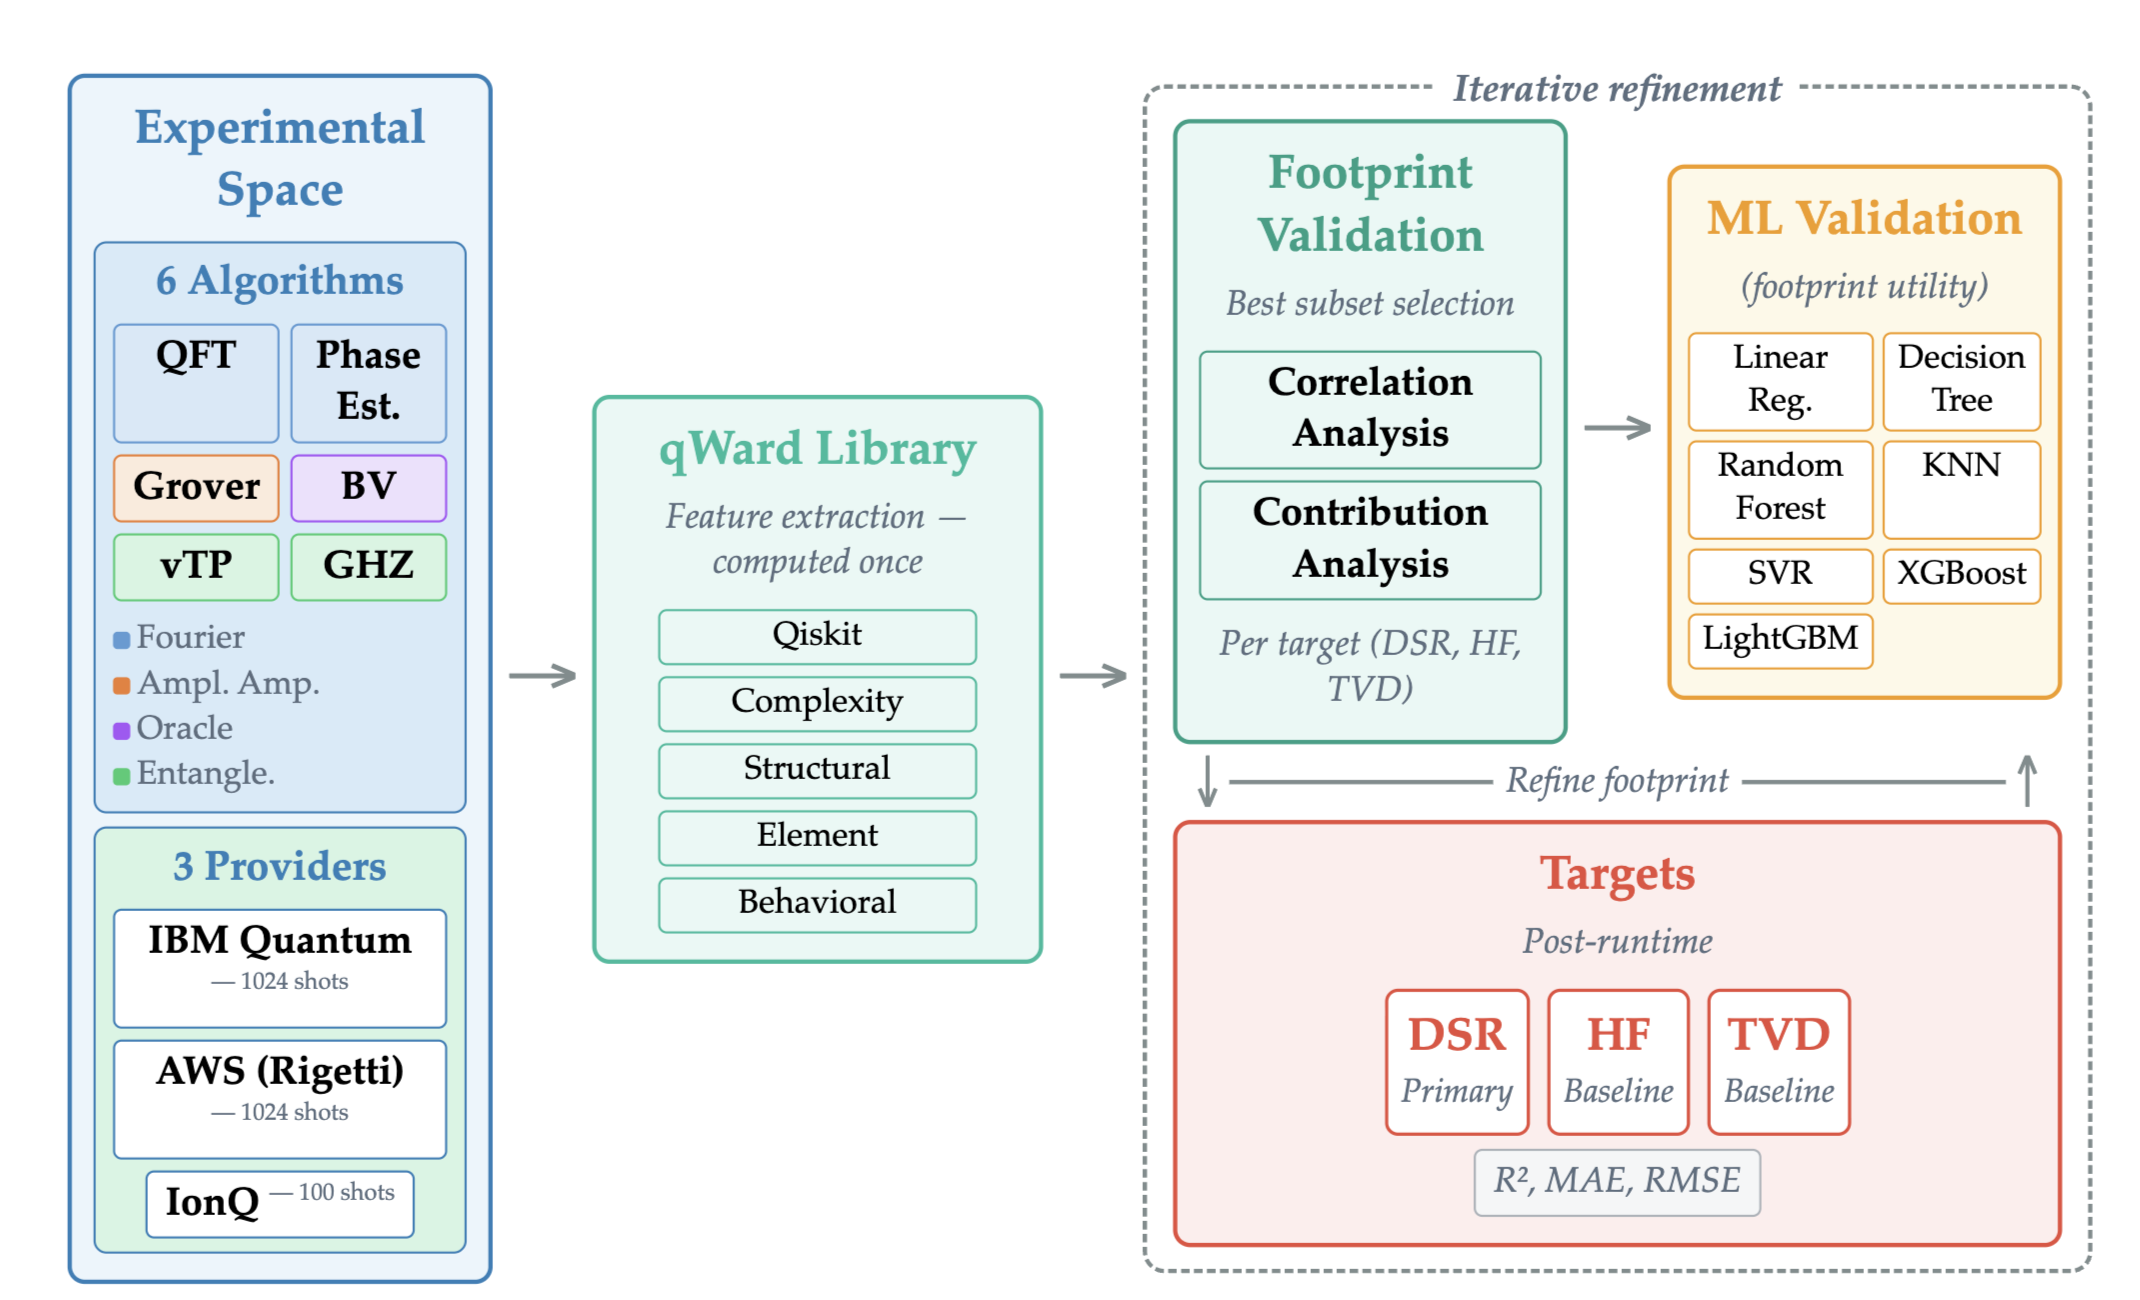
\includegraphics[width=1\textwidth]{proposal.png}
    \caption{Overview of the predictive framework. The circuit footprint calculated by qWard is used as input to supervised regression models that estimate execution quality (DSR, HF, TVD).}
    \label{fig:framework-overview}
\end{figure*}

Based on these findings, the next step is to formalize the circuit footprint (Section~\ref{section:introduction}), calculated by qWard in Figure~\ref{fig:framework-overview}, into a predictive pipeline. This requires defining how success is measured for each algorithm and justifying the choice of DSR, HF, and TVD as the post-runtime targets (shown in the Targets block) introduced earlier.

Before proceeding, it is worth noting that the footprint is not strictly a property of the logical circuit. Because the metrics are computed after transpilation, two-qubit gate counts and circuit depth already absorb the device's coupling map, basis-gate set, and routing decisions. The footprint therefore characterizes the circuit compiled for a specific target device, and Section~\ref{subsec:scope} returns to this nuance as part of the study delimitations.

Regarding the success function, one crucial aspect to consider is that the six target algorithms differ in how their outputs are evaluated. In previous studies, we identified that validation can be performed per shot, per job, or per batch. Algorithms such as vTP or GO produce deterministic outcomes that can be evaluated per shot, meaning that the result either matches the expected value or does not. In contrast, QFT-based algorithms require an analysis of the output probability distribution, making evaluation at the job or batch level more appropriate.

To address the need for a unified and interpretable success criterion, this thesis adopts the DSR, a post-runtime metric currently under peer review at IEEE Quantum Week 2026, as its primary evaluation target, complemented by HF and TVD for comparative analysis. The DSR is defined by Equation~\eqref{eq:dsr}.

\begin{equation}
\label{eq:dsr}
DSR = \text{clip}\!\left(\frac{\bar{p}_{exp} - p_{comp}}{\bar{p}_{exp} + p_{comp}},\ 0,\ 1\right)
\end{equation}

\noindent Let $\mathcal{C} : \{0,1\}^n \to \mathbb{Z}_{\geq 0}$ denote the histogram returned by a quantum job, with total shots $S = \sum_{x} \mathcal{C}(x)$ and probability of outcomes $p_x = \mathcal{C}(x)/S$. Given the set of expected outcomes $E$ with cardinality $K = |E|$, the terms are defined in Equation~\eqref{eq:dsr_terms}.

\begin{equation}
\label{eq:dsr_terms}
\bar{p}_{\text{exp}} = \frac{1}{K}\sum_{x \in E} p_x, \qquad
p_{\text{comp}} = \max_{x \notin E}\; p_x
\end{equation}

\noindent That is, $\bar{p}_{exp}$ is the mean probability per expected outcome and $p_{comp}$ is the probability of the strongest competing (non-expected) state. Since $\bar{p}_{exp} \geq 0$ and $p_{comp} \geq 0$, the fraction in Equation~\eqref{eq:dsr} is bounded in $[-1, 1]$; the clip affects only the cases where $p_{comp} > \bar{p}_{exp}$, collapsing the result to zero. The DSR adopts the Michelson contrast formulation \cite{michelsonInterferenceMethods_1890, michelsonStudiesOptics_1927}, which provides three desirable properties: \emph{(i)} scale invariance, since $S$ cancels out and the score depends only on relative strengths; \emph{(ii)} a bounded range in $[0, 1]$; and \emph{(iii)} sensitivity to the dominance of the expected outcome over the strongest competitor. In practical terms, if $\mathrm{DSR} = d$ (for $d < 1$), the signal-to-competitor ratio satisfies $\bar{p}_{exp} / p_{comp} = (1 + d)/(1 - d)$; for example, $d = 0.8$ corresponds to a ratio $9{:}1$. Edge cases are handled by convention: $S = 0$ or $E = \emptyset$ yields $\mathrm{DSR} = 0$; if all observed states belong to $E$, then $p_{comp} = 0$ and $\mathrm{DSR} = 1$.

The DSR has known limitations. Because it compares only against the single strongest competitor, it is insensitive to how probability mass is distributed among all non-expected states. It also requires knowledge of the expected output states, restricting its applicability to algorithms with a known ground truth. Furthermore, for algorithms that produce multiple expected states, the use of the mean $\bar{p}_{exp}$ can mask cases where some expected states are well-resolved while others are lost in noise. Finally, scale invariance holds in practice only under sufficient sampling; with very few shots, the histogram may not accurately reflect the algorithm's output distribution.

Although all three metrics require knowledge of the expected output states, they differ in what they measure. HF and TVD compare the full observed probability distribution with the ideal one, capturing how faithfully the hardware reproduces the entire output profile. The DSR, in contrast, focuses exclusively on the contrast between the target states and the strongest competitor, aiming to answer whether the algorithm's targeted output emerges above the noise.

Importantly, the QAQS framework does not depend on the superiority of DSR over established metrics. Because HF and TVD serve as co-equal prediction targets throughout the pipeline, the footprint validation and the predictive models remain valid regardless of which metric proves most informative. If DSR turns out to be a weaker predictor than HF or TVD, the core contribution---the circuit footprint as a quality model---is still validated through the established metrics, and DSR would simply be documented as a complementary measure with a more limited scope.

Recent studies provide evidence that ML models trained in specific circuit families can generalize to unseen configurations that preserve the structural characteristics of the original primitive. Vadali et al. \cite{vadaliQuantumCircuitFidelity_2024} demonstrated that models trained on simpler circuits can predict the fidelity of circuits with higher degrees of entanglement and non-Clifford gates than those present in the training set. Similarly, Ravi et al. \cite{raviAdaptiveJobResource_2021} showed that the fidelity predictions derived from the features of the circuit compiled are generalized to a diverse set of quantum applications on IBM hardware. Moreover, Hopf et al. \cite{hopfImprovingFiguresMerit_2025} proposed an ML-based figure of merit that predicts execution quality without running the circuit, achieving a 49\% correlation improvement over the state of the art. Taken together, these findings support the premise that models can generalize to unseen configurations within the same primitive, as proposed in this thesis.

To further enhance generalizability, the dataset is obtained by running the algorithms in three different quantum services, shown in the Experimental Space block of Figure~\ref{fig:framework-overview} and detailed in Section~\ref{subsec:scope}. This approach tests whether pre-runtime metrics demonstrate predictive value while expanding the diversity of noise profiles and connectivity constraints in the training data.

The footprint then feeds into the Footprint Validation block of Figure~\ref{fig:framework-overview}, where a correlation and contribution analyze selects the most predictive subset of metrics per target. The selected footprint is forwarded to the ML Validation module, which trains the seven classical supervised regression models specified in Section~\ref{subsec:scope} in order to predict the execution quality (\ref{h:1}). The results of the targets are finally sent through the "Refine footprint" loop, closing the iterative refinement cycle.

\subsection{Dataset Structure}
\label{subsec:dataset-validation}

The dataset is organized into four feature groups, each capturing a distinct aspect of the quantum circuit structure. Table~\ref{tab:dataset-structure} summarizes these groups.

\begin{table}[ht]
\renewcommand{\arraystretch}{1.1}
\centering
\caption{Feature groups and some representative variables on each category.}
\label{tab:dataset-structure}
\footnotesize
\begin{tabular}{|p{2cm}|p{3cm}|p{5.8cm}|}
\hline
\textbf{Feature Group} & \textbf{When Collected} & \textbf{Representative Variables} \\
\hline
Pre-runtime metrics & After transpilation, before execution & Circuit depth, width, gate count, CNOT count, multi-qubit ratio, entangling gate density, Halstead volume, critical depth, liveness, parallelism, magic, coherence, sensitivity \\
\hline
Backend calibration & Before execution (from provider API) & Median single-qubit gate error, median two-qubit gate error, median readout error, median $T_1$, median $T_2$, number of operational qubits \\
\hline
Post-runtime metrics (targets) & After execution & DSR, Hellinger fidelity, TVD, success rate, entropy, dominant outcome probability \\
\hline
Gate error characterization & Before execution (from provider API) & Per-gate error rates reported by the backend for the specific qubits used in the transpiled circuit (e.g., CX error on qubit pair [0,1], single-qubit error on qubit 3) \\
\hline
\end{tabular}
\end{table}

The inclusion of gate error characterization as a separate feature group is to explore the impact of hardware noise on quantum software quality. Gate depth and gate-specific error rates are known to propagate across circuit layers; by recording per-gate error rates for the specific qubits allocated during transpilation, the dataset enables an analysis of whether noise-aware features improve prediction beyond what the circuit-only footprint captures implicitly through transpilation artifacts (e.g., inserted SWAP gates).

\subsection{Validation Plan}

The validation procedure is structured to systematically evaluate each algorithmic paradigm under controlled scaling conditions. For each of the three paradigms, the plan specifies:

\begin{enumerate}
\item \textbf{Fourier-based (QFT, PE).} Circuits are scaled by progressively increasing the number of qubits, which in turn increases pre-runtime metrics such as gate count, CNOT count, circuit depth, and width. Scaling continues until the maximum size for which the backend maintains a post-runtime metric (e.g., fidelity) with a score of at least $1\%$ of getting a positive answer.

\item \textbf{Oracle-based (GO, BV).} In addition to qubit scaling, Grover's algorithm varies the number and Hamming weight of marked states, producing configurations that stress different aspects of the oracle structure. BV varies the secret bit-string length. Each configuration is executed under the same multi-job protocol described above.

\item \textbf{Entanglement-based (vTP, GHZ).} The vTP protocol scales the payload size from 1 to $n$ qubits, injecting random single-qubit gates per payload qubit. GHZ follows a volumetric growth strategy that increases both qubit count and gate depth by appending random single-qubit and two-qubit operations (for entanglement preparation) drawn from the backend's native gate set. The GHZ random-circuit variant serves as the control group for Hypothesis~\ref{h:4}, enabling a direct comparison between paradigm-specific scaling and random-circuit-based hardware benchmarking.
\end{enumerate}

For all paradigms, the dataset records the four feature groups described in Table~\ref{tab:dataset-structure}. All circuits will be executed using optimization level 3, and the pre-runtime metrics will be evaluated following the transpilation stage. The validation strategy employs a temporal split in which models are trained on earlier executions and validated against subsequent executions collected on different calibration cycles. In addition, the study compares the precision between models trained in paradigm-specific circuits and models trained on the GHZ random-circuit baseline, testing whether structured algorithms provide a richer predictive signal than volumetric random benchmarks (\ref{h:4}).

\section{Scope and Delimitations}
\label{subsec:scope}

Because this study relies on execution data from a heterogeneous set of quantum platforms, the experimental design targets three providers, specifically superconducting-qubit systems from IBM and Rigetti, and trapped-ion hardware from IonQ. However, it should be emphasized that validation on physical devices is tightly constrained by available research funding and cloud access grants, which may reduce the amount of real-hardware execution data relative to simulator-produced data.

Given the vast variety of algorithms available, this study is restricted to those for which the expected output quantum states are known a priori, since the DSR requires this information in order to compute the corresponding success score. Algorithms whose ideal output is a broad probability distribution without a discrete set of dominant states, such as variational algorithms, are excluded from the scope of this work. The training and testing datasets will be constructed by executing the six algorithms described in Section~\ref{subsec:paradigms} (Table~\ref{tab:paradigms}) on real quantum hardware in the three target providers. For each algorithm, the circuit will be progressively scaled until the DSR indicates that the hardware can no longer produce a meaningful output, thus defining the practical limit of each provider for that algorithm.

Regarding the training data, the scope is restricted to pre-runtime metrics derived from a static analysis of the quantum circuit representation (after its transpilation) and before its execution. The construction of the "circuit footprint" will be driven by a correlation analysis designed to identify the specific subset of metrics that exhibit the strongest predictive power for execution quality.

Because transpilation is target-dependent, the resulting footprint already encodes hardware characteristics implicitly (e.g., additional SWAP gates due to connectivity constraints or different basis-gate decompositions). Whether this implicit encoding is adequate for reliable prediction across providers, or whether it is necessary to incorporate explicit backend calibration, remains an open question. This issue motivates the secondary analysis described below and is formally examined in Hypothesis~\ref{h:3}.

To investigate the impact of the hardware context, the study will also evaluate two hardware-aware variants. The first uses only explicit backend calibration features, such as median gate error rates and/or $T_1$/$T_2$ coherence times, all of which are publicly available before execution. The second is a mixed configuration that combines these calibration features with the footprint of the circuit alone. Both variants will be compared against the circuit-only footprint, which beyond the implicit structural encoding after transpilation discussed above contains no explicit backend features, to characterize the extent to which hardware context is necessary for cross-provider prediction (\ref{h:3}).

Because the available dataset is limited, the models will be trained using all the execution records collected. Validation will be performed using newly generated execution data that is not used during model construction. The predicted quality metrics will then be compared with the observed outcomes of these new executions.

Regarding the random-circuit comparison (\ref{h:4}), the underlying rationale is that each algorithmic paradigm produces a distinct structural scaling shape---in terms of depth profile, entanglement pattern, and gate composition---that is not uniformly sampled by the benchmarking using random circuit. Consequently, paradigm-specific benchmark executions may reveal hardware-dependent performance that are not captured by randomly generated workloads, thereby providing empirically guidance regarding which backend is most appropriate for a target algorithm.

Finally, with respect to the predictive modeling component, this research focuses on the application of classical machine learning algorithms rather than deep learning or quantum machine learning approaches. This choice is justified because the input vector and target variables are structured data, avoiding the need for deep architectures that are typically required for unstructured data such as text or images. The study will evaluate a comprehensive suite of regression models, including Linear Regression, Decision Tree Regression, Random Forest, K-Nearest Neighbors (KNN), Support Vector Machine Regression (SVR), and Gradient Boosting algorithms such as XGBoost and LightGBM. The best algorithm selection will be based on the Coefficient of Determination ($R^2$), Mean Absolute Error (MAE), and Root Mean Squared Error (RMSE), with a minimum score of $R^2 \geq 0.80$ and the goal of minimizing the MAE and RMSE respectively.

\section{Expected Contributions}
\label{section:contributions}

The central doctoral contribution of this thesis is the \textbf{Quality-Aware Quantum Software (QAQS) framework}, a pre-runtime quality model for quantum software that links a circuit's structural properties to its expected execution outcomes. Contributions are listed below, organized from conceptual foundations to software artifacts.

\begin{enumerate}

\item \textbf{Pre/Post-runtime Metric Classification:} A temporal metric taxonomy, derived from the systematic mapping study (Section~\ref{subsection:sms}), that distinguishes between pre-runtime metrics (obtained through static analysis) and post-runtime metrics (obtained from execution results). This classification provides the conceptual foundation for QAQS.
\label{c:classification}

\item \textbf{DSR Metric:} A distribution-aware post-runtime metric, described in Section~\ref{section:qaqs}, that quantifies the contrast between the expected outcome states and the strongest competing state. Paper submitted to IEEE Quantum Week 2026 (under review).
\label{c:dsr}

\item \textbf{Circuit Footprint:} An empirically validated feature vector of pre-runtime metrics (Section~\ref{section:introduction}) selected through iterative correlation and contribution analysis per target. The footprint condenses a quantum circuit into a compact representation suitable for quality prediction.
\label{c:footprint}

\item \textbf{qWard Library:} An open-source Python library \cite{marquezQwardUnifiedToolkit_2025, QiskitqwardFrameworkAnalyzing} for automated metric extraction from quantum circuits (Section~\ref{subsection:qward}). qWard operationalizes the metric classification by providing 30+ pre-runtime and 8+ post-runtime metrics.
\label{c:qward}

\item \textbf{Open Datasets:} Three publicly available datasets \cite{data_1, data_2} published in IEEE Dataport, comprising 292 and 1,281 QPU executions, respectively, together with a forthcoming multi-paradigm, multi-provider validation dataset covering six algorithms on IBM, Rigetti, and IonQ hardware. These datasets, described in Section~\ref{subsection:vtp}, provide the empirical foundation for the predictive framework.
\label{c:dataset1}

\item \textbf{Predictive Pipeline (QAQS):} A software tool that integrates metric extraction via qWard, footprint validation, and ML-based prediction into a unified pipeline, as described in Section~\ref{section:qaqs} and Figure~\ref{fig:framework-overview}.
\label{c:framework}

\end{enumerate}

\subsection{Derived Subproducts}

This research has also produced tangible outcomes in the form of undergraduate theses co-supervised within the scope of the qWard project at Universidad de los Andes, demonstrating the framework's applicability in educational settings.

\begin{enumerate}

\item Torres Bermejo \cite{torresBermejoVisualizationsPostRuntime_2025} developed a visualization module for post-runtime quantum circuit information, integrated into qWard as part of the Visualizer component.

\item Baldion Castillo \cite{baldionCastilloPreRuntimeMetrics_2026} implemented a pre-runtime metric extraction pipeline and validated its predictive power for quantum execution success rates using Grover's algorithm as a case study.

\item Rodr\'{i}guez Castillo \cite{rodriguezCastilloScalabilityQuantum_2026} analyzed the scalability behavior of quantum algorithms implemented as circuits and subroutines, providing empirical evidence on how the circuit structure evolves with the size of the problem.

\end{enumerate}

\section{Research Plan}
\label{section:work}

This section presents the thesis research plan, organized as a series of phases that directly operationalize the GBMF and GQM paradigm described in Section~\ref{section:methodology}. Each phase represents a discrete unit of work with a clear objective, estimated duration, and acceptance criteria.

The research plan is presented as ten phases, three of which have been completed, two are currently in progress, and five remain to be executed.

\setlength{\LTleft}{0pt}
\begin{longtable}{@{}p{\textwidth}@{}}
    \toprule
    \textbf{Phase 1: GQM Conception -- Goal and Question Definition} \label{p:1} \hfill \textbf{Status: DONE} \\
    \textit{Estimation:} 3 Months \newline
    \textbf{Related Goals:} Objective \ref{o:1} \newline
    \textbf{Description:} Following the Goal-Based Measurement Framework (GBMF), this phase executes the first two steps of the GQM paradigm. Through a systematic mapping review, we identify the core problem---the unreliability of NISQ hardware---to establish the General Objective (the ``Goal'') and derive the primary Research Question (the ``Question'') assessing the predictive power of pre-runtime metrics. \newline
    \textbf{Tasks:}
    \begin{enumerate}[label=T1.\arabic*, ref=T1.\arabic*, font=\bfseries, leftmargin=3.5em, labelindent=0pt, itemindent=0pt, labelsep=0.5em, noitemsep, topsep=0pt]
        \item \label{p1:t1} Conduct Systematic Mapping Review.
    \end{enumerate}
    \textbf{Acceptance Criteria:}
    \begin{itemize}[leftmargin=1.5em, labelindent=0pt, itemindent=0pt, noitemsep, topsep=0pt]
        \item Systematic mapping study completed and research gaps identified.
        \item Preliminary findings published and initial hypotheses validated.
    \end{itemize}
    \textbf{Result:}
    \begin{itemize}[leftmargin=1.5em, labelindent=0pt, itemindent=0pt, noitemsep, topsep=0pt]
        \item Poster "Quality concerns when integrating quantum and classical computing: a systematic mapping study" published in CIbSE 2025. \cite{marquezQualityConcernsWhena_2025}
    \end{itemize} \\
    \midrule
    
    \textbf{Phase 2: Metric Specification and Tooling (The ``M'' in GQM)} \label{p:2} \hfill \textbf{Status: DONE} \\
    \textit{Estimation:} 6 Months \newline
    \textbf{Related Goals:} Objective \ref{o:1} \newline
    \textbf{Description:} Executing the third step of GQM, this phase identifies the specific metrics required to answer the Research Question. We classify quantum circuit attributes temporally into internal (pre-runtime) and external (post-runtime) metrics, following the GBMF distinction between measures and prediction systems. To automate the systematic extraction of the ``circuit footprint,'' we develop the qWard library as the measurement tool. \newline
    \textbf{Tasks:}
    \begin{enumerate}[label=T2.\arabic*, ref=T2.\arabic*, font=\bfseries, leftmargin=3.5em, labelindent=0pt, itemindent=0pt, labelsep=0.5em, noitemsep, topsep=0pt]
        \item \label{p2:t1} Design the qWard library.
        \item \label{p2:t2} Create project structure, docs and CI-CD integrations.
        \item \label{p2:t3} Create Scanner, and Pre-runtime classes.
        \item \label{p2:t4} Create Post-runtime classes.
        \item \label{p2:t5} Create Visualization classes.
        \item \label{p2:t6} Implement first batch of Pre-runtime metrics.
        \item \label{p2:t7} Implement first batch of Post-runtime metrics.
        \item \label{p2:t8} Prepare documentation.
        \item \label{p2:t9} Prepare poster and paper.
    \end{enumerate}
    \textbf{Acceptance Criteria:}
    \begin{itemize}[leftmargin=1.5em, labelindent=0pt, itemindent=0pt, noitemsep, topsep=0pt]
        \item Alpha version of the qWard library developed and functional.
        \item Metric extraction capabilities implemented and tested.
    \end{itemize}
    \textbf{Result:}
    \begin{itemize}[leftmargin=1.5em, labelindent=0pt, itemindent=0pt, noitemsep, topsep=0pt]
        \item Paper and Poster presented at CHILECON 2025 \cite{marquezQwardUnifiedToolkit_2025}. Proceedings forthcoming.
    \end{itemize} \\
    \midrule
    
    \textbf{Phase 3: Empirical Pilot Study (vTP)} \label{p:3} \hfill \textbf{Status: DONE} \\
    \textbf{Estimation:} 6 Months \newline
    \textbf{Related Goals:} Hypothesis \ref{h:1} \newline
    \textbf{Description:} Conduct the first empirical study to gather ground-truth data under controlled conditions. Using the vTP, this phase validates that the internal attributes (pre-runtime metrics) defined in \hyperref[p:2]{Phase~2} exhibit a statistical correlation with external attributes (post-runtime success rate), providing initial evidence for the prediction system proposed by the GBMF. \newline
    \textbf{Tasks:}
    \begin{enumerate}[label=T3.\arabic*, ref=T3.\arabic*, font=\bfseries, leftmargin=3.5em, labelindent=0pt, itemindent=0pt, labelsep=0.5em, noitemsep, topsep=0pt]
        \item \label{p3:t1} Execute Pilot Experiment (vTP).
    \end{enumerate}
    \textbf{Acceptance Criteria:}
    \begin{itemize}[leftmargin=1.5em, labelindent=0pt, itemindent=0pt, noitemsep, topsep=0pt]
        \item Pilot experiment (vTP) executed on IBM and Rigetti.
        \item Analysis confirming correlation between structure and reliability completed.
    \end{itemize}
    \textbf{Result:}
    \begin{itemize}[leftmargin=1.5em, labelindent=0pt, itemindent=0pt, noitemsep, topsep=0pt]
        \item Paper "A Teleportation Protocol Variant for Single-QPU Benchmarking" accepted in IEEE Access \cite{ieeevTp2025}.
        \item QPU executions on IBM and AWS (Rigetti Ankaa-3).
        \item Open dataset published on IEEE Dataport \cite{data_1}.
    \end{itemize} \\
    \midrule

    \textbf{Phase 4: Data Collection and Experimentation} \label{p:4} \hfill \textbf{Status: IN PROGRESS} \\
    \textit{Estimation:} 3 Months \newline
    \textbf{Related Goals:} Hypothesis \ref{h:1}, Objective \ref{o:1} \newline
    \textbf{Description:} Populate the measurement dataset with both the pre-runtime ``footprint'' data (internal attributes) and the post-runtime execution results (external attributes) that serve as the ground truth for the prediction system. This phase executes the six target algorithms described in Section~\ref{subsec:scope} across IBM, Rigetti, and IonQ quantum providers. \newline
    \textbf{Tasks:}
    \begin{enumerate}[label=T4.\arabic*, ref=T4.\arabic*, font=\bfseries, leftmargin=3.5em, labelindent=0pt, itemindent=0pt, labelsep=0.5em, noitemsep, topsep=0pt]
        \item \label{p4:t1} Prepare the 6 target algorithms for execution.
        \item \label{p4:t2} Execute algorithms on IBM backend and collect results.
        \item \label{p4:t3} Execute algorithms on Rigetti backend and collect results.
        \item \label{p4:t4} Execute algorithms on IonQ backend and collect results.
        \item \label{p4:t5} Consolidate results and perform data cleaning.
    \end{enumerate}
    \textbf{Acceptance Criteria:}
    \begin{itemize}[leftmargin=1.5em, labelindent=0pt, itemindent=0pt, noitemsep, topsep=0pt]
        \item Dataset generated from 6 target algorithms across 3 quantum providers.
        \item Data cleaning and preprocessing pipeline implemented.
        \item CSV file with consolidated execution data delivered.
    \end{itemize}
    \textbf{Result:}
    \begin{itemize}[leftmargin=1.5em, labelindent=0pt, itemindent=0pt, noitemsep, topsep=0pt]
        \item Open dataset with 1,281 QPU executions (Grover, QFT, vTP) across IBM Quantum and AWS (Rigetti Ankaa-3) published on IEEE Dataport \cite{data_2}.
        \item IonQ execution and BV and GHZ data collection pending.
    \end{itemize} \\
    \midrule

    \textbf{Phase 4b: DSR Theoretical Foundation and Validation} \label{p:4b} \hfill \textbf{Status: IN PROGRESS} \\
    \textit{Estimation:} 16 Weeks (June--September 2026, non-blocking, parallel with Phases 5--7) \newline
    \textbf{Related Goals:} Hypothesis \ref{h:1}, Objective \ref{o:1} \newline
    \textbf{Description:} Formalize the theoretical foundations of DSR as a distribution-aware metric for validating quantum algorithm outputs. This work will be conducted as part of a research internship at The Catholic University of America under the supervision of Daniel Sierra-Sosa, and includes the empirical validation of DSR against established fidelity metrics across multiple quantum providers. This phase runs independently and does not block the main research pipeline. \newline
    \textbf{Tasks:}
    \begin{enumerate}[label=T4b.\arabic*, ref=T4b.\arabic*, font=\bfseries, leftmargin=3.5em, labelindent=0pt, itemindent=0pt, labelsep=0.5em, noitemsep, topsep=0pt]
        \item \label{p4b:t1} Formalize the DSR metric definition and its four variants (Michelson, ratio, log-ratio, normalized margin).
        \item \label{p4b:t2} Conduct empirical comparison of DSR against HF and TVD across IBM and Rigetti backends.
        \item \label{p4b:t3} Analyze DSR sensitivity to circuit scale, transpilation optimization level, and hardware noise.
        \item \label{p4b:t4} Prepare and submit the research paper.
        \item \label{p4b:t5} Integrate DSR computation into the qWard library.
    \end{enumerate}
    \textbf{Acceptance Criteria:}
    \begin{itemize}[leftmargin=1.5em, labelindent=0pt, itemindent=0pt, noitemsep, topsep=0pt]
        \item DSR formally defined with theoretical justification.
        \item Empirical validation completed on 1,281 QPU executions \cite{data_2}.
        \item DSR integrated into qWard as a post-runtime metric.
    \end{itemize}
    \textbf{Result:}
    \begin{itemize}[leftmargin=1.5em, labelindent=0pt, itemindent=0pt, noitemsep, topsep=0pt]
        \item Journal paper submitted.
        \item Research internship at The Catholic University of America pending.
    \end{itemize} \\
    \midrule

    \textbf{Phase 5: Success Function Specification} \label{p:5} \hfill \textbf{Status: TO DO} \\
    \textit{Estimation:} 1 Month \newline
    \textbf{Related Goals:} Hypothesis \ref{h:1}, Objective \ref{o:1} \newline
    \textbf{Description:} Refine the ``M'' in GQM by formalizing the success function---the external attribute that serves as the prediction target---for each of the six target algorithms. Since determining success varies by algorithm paradigm, this phase focuses on defining the evaluation criteria and implementing the corresponding logic in qWard. \newline
    \textbf{Tasks:}
    \begin{enumerate}[label=T5.\arabic*, ref=T5.\arabic*, font=\bfseries, leftmargin=3.5em, labelindent=0pt, itemindent=0pt, labelsep=0.5em, noitemsep, topsep=0pt]
        \item \label{p5:t1} Investigate success criteria used in adjacent disciplines, for example in cryptography. 
        \item \label{p5:t2} Define success criteria for QFT-based algorithms.
        \item \label{p5:t3} Define success criteria for GO.
        \item \label{p5:t4} Define success criteria for BV.
        \item \label{p5:t5a} Define success criteria for entanglement-based algorithms (vTP, GHZ).
        \item \label{p5:t5} Implement success functions in qWard library.
    \end{enumerate}
    \textbf{Acceptance Criteria:}
    \begin{itemize}[leftmargin=1.5em, labelindent=0pt, itemindent=0pt, noitemsep, topsep=0pt]
        \item Success function defined and implemented for each of the 6 target algorithms.
        \item Implementation of success functions in qWard library.
    \end{itemize} \\
    \midrule
    
    \textbf{Phase 6: Feature Engineering and Correlation Analysis} \label{p:6} \hfill \textbf{Status: TO DO} \\
    \textit{Estimation:} 1 Month \newline
    \textbf{Related Goals:} Hypothesis \ref{h:1}, Objective \ref{o:1} \newline
    \textbf{Description:} Define the "Quantum Circuit Footprint" feature vector by performing correlation analysis (Spearman), contribution analysis (permutation importance, SHAP), and multicollinearity removal (VIF) per target (DSR, HF, TVD). Compare prediction results across three input configurations (circuit-only, hardware-only, and mixed) to assess the role of backend context. \newline
    \textbf{Tasks:}
    \begin{enumerate}[label=T6.\arabic*, ref=T6.\arabic*, font=\bfseries, leftmargin=3.5em, labelindent=0pt, itemindent=0pt, labelsep=0.5em, noitemsep, topsep=0pt]
        \item \label{p6:t1} Perform exploratory data analysis: distributions, outliers, and multicollinearity among candidate pre-runtime and hardware metrics.
        \item \label{p6:t2} Run Spearman correlation analysis between candidate metrics and post-runtime targets.
        \item \label{p6:t3} Conduct contribution analysis (permutation importance, SHAP) to rank feature predictive signal.
        \item \label{p6:t4} Select the optimal pre-runtime metric set for the "Quantum Circuit Footprint" and handle multicollinearity (e.g., VIF-based removal).
        \item \label{p6:t5} Compare prediction results obtained with pre-runtime-only, hardware-only, and mixed input configurations.
    \end{enumerate}
    \textbf{Acceptance Criteria:}
    \begin{itemize}[leftmargin=1.5em, labelindent=0pt, itemindent=0pt, noitemsep, topsep=0pt]
        \item Correlation and contribution analyses completed for the candidate metrics and target variables (DSR, HF, TVD).
        \item "Quantum Circuit Footprint" defined with explicit justification for each included pre-runtime metric.
        \item Multicollinearity addressed and documented.
        \item Prediction results compared across pre-runtime-only, hardware-only, and mixed configurations.
    \end{itemize} \\
    \midrule
    
    \textbf{Phase 7: Prediction System Construction} \label{p:7} \hfill \textbf{Status: TO DO} \\
    \textit{Estimation:} 3 Months \newline
    \textbf{Related Goals:} Hypothesis \ref{h:1}, Objective \ref{o:2} \newline
    \textbf{Description:} Construct the GBMF prediction system by training and tuning the seven supervised regression models described in Section~\ref{subsec:scope}. In measurement theory, a prediction system uses a mathematical model to predict an attribute of a future entity; here, the models map the internal attributes (the circuit footprint) to external attributes (execution quality). Integrate these models into the QAQS framework. \newline
    \textbf{Tasks:}
    \begin{enumerate}[label=T7.\arabic*, ref=T7.\arabic*, font=\bfseries, leftmargin=3.5em, labelindent=0pt, itemindent=0pt, labelsep=0.5em, noitemsep, topsep=0pt]
        \item \label{p7:t1} Implement training pipeline for all regression models.
        \item \label{p7:t2} Train and tune Linear Regression and Decision Tree models.
        \item \label{p7:t3} Train and tune Random Forest and K-Nearest Neighbors models.
        \item \label{p7:t4} Train and tune Support Vector Regression model.
        \item \label{p7:t5} Train and tune Gradient Boosting models including XGBoost and LightGBM.
        \item \label{p7:t6} Integrate model generation and inference capabilities into qWard.
        \item \label{p7:t7} Implement evaluation metrics for model performance assessment.
    \end{enumerate}
    \textbf{Acceptance Criteria:}
    \begin{itemize}[leftmargin=1.5em, labelindent=0pt, itemindent=0pt, noitemsep, topsep=0pt]
        \item All seven regression models trained and tuned.
        \item Models integrated into the QAQS framework.
        \item Model generation and inference integrated into qWard.
        \item Performance evaluation using $R^2$, MAE, and RMSE implemented.
    \end{itemize} \\
    \midrule
    
    \textbf{Phase 8: Measurement Validation and Empirical Analysis} \label{p:8} \hfill \textbf{Status: TO DO} \\
    \textit{Estimation:} 2 Months \newline
    \textbf{Related Goals:} Hypothesis \ref{h:2}, \ref{h:3}, \ref{h:4}; Objective \ref{o:3}, \ref{o:4} \newline
    \textbf{Description:} Close the GBMF loop by validating predictions against ground-truth data from new QPU executions. This phase evaluates generalization (\ref{h:2}), cross-provider transferability (\ref{h:3}), and paradigm-specific vs.\ random-circuit hardware characterization (\ref{h:4}). \newline
    \textbf{Tasks:}
    \begin{enumerate}[label=T8.\arabic*, ref=T8.\arabic*, font=\bfseries, leftmargin=3.5em, labelindent=0pt, itemindent=0pt, labelsep=0.5em, noitemsep, topsep=0pt]
        \item \label{p8:t1} Execute target algorithms on real hardware to collect validation data.
        \item \label{p8:t2} Compare predicted vs.\ observed quality metrics.
        \item \label{p8:t3} Compare results across pre-runtime-only, hardware-only, and mixed configurations.
        \item \label{p8:t4} Compare paradigm-trained models against random-circuit-trained models.
        \item \label{p8:t5} Quantify predictive power and document limitations.
    \end{enumerate}
    \textbf{Acceptance Criteria:}
    \begin{itemize}[leftmargin=1.5em, labelindent=0pt, itemindent=0pt, noitemsep, topsep=0pt]
        \item Validation dataset from new QPU executions collected.
        \item Generalization within paradigms validated (\ref{h:2}).
        \item Cross-provider prediction assessed across input configurations (\ref{h:3}).
        \item Paradigm-specific vs.\ random-circuit characterization compared (\ref{h:4}).
        \item Results reported using $R^2$, $MAE$, and $RMSE$.
    \end{itemize} \\
    \midrule
    
    \textbf{Phase 9: Thesis Synthesis and Dissemination} \label{p:9} \hfill \textbf{Status: TO DO} \\
    \textit{Estimation:} 2 Months \newline
    \textbf{Related Goals:} General Objective \newline
    \textbf{Description:} Synthesize research findings into the doctoral dissertation, submit final results for evaluation, and prepare for the thesis defense. \newline
    \textbf{Tasks:}
    \begin{enumerate}[label=T9.\arabic*, ref=T9.\arabic*, font=\bfseries, leftmargin=3.5em, labelindent=0pt, itemindent=0pt, labelsep=0.5em, noitemsep, topsep=0pt]
        \item \label{p9:t1} Write and structure the thesis chapters based on research findings.
        \item \label{p9:t2} Submit draft to advisors and incorporate feedback.
        \item \label{p9:t3} Prepare qWard and Framework documentation for public release.
        \item \label{p9:t4} Create defense presentation slides.
        \item \label{p9:t5} Conduct thesis defense.
    \end{enumerate}
    \textbf{Acceptance Criteria:}
    \begin{itemize}[leftmargin=1.5em, labelindent=0pt, itemindent=0pt, noitemsep, topsep=0pt]
        \item Doctoral dissertation written and defended.
        \item qWard and Framework documentation finalized for public release.
    \end{itemize} \\
    \bottomrule
    \end{longtable}

\section{Timeline}

Figure \ref{fig:gantt} presents the Gantt chart for the thesis research plan. The timeline spans 27 months, divided into three states. The first state covers 15 months of completed foundational work, including the GQM conception (\hyperref[p:1]{Phase~1}), metric specification and tooling (\hyperref[p:2]{Phase~2}), and the empirical pilot study (\hyperref[p:3]{Phase~3}). The second state represents the current collection of empirical data from multiple quantum providers (\hyperref[p:4]{Phase~4}). In addition, \hyperref[p:4b]{Phase~4b} runs independently from June to September 2026 as a non-blocking research internship dedicated to the DSR theoretical foundation and validation. The third state includes the remaining 9 months of future work, which involves specifying success functions, performing correlation analysis, constructing the prediction system, validating the measurements, and synthesizing the thesis document.

\definecolor{barblue}{RGB}{153,204,254}
\definecolor{barfuture}{HTML}{6c757d}
\definecolor{groupblue}{RGB}{51,102,254}
\definecolor{bardone}{RGB}{34,139,34}
\definecolor{barinprogress}{RGB}{255,193,7}
\definecolor{groupinprogress}{RGB}{255,152,0}

\begin{figure*}[ht]
\centering
\begin{ganttchart}[
    canvas/.append style={fill=none, draw=black!5, line width=.75pt},
    hgrid style/.style={draw=black!5, line width=.75pt},
    vgrid={*1{draw=black!5, line width=.75pt}},
    today=16,
    today rule/.style={
      draw=black!64,
      dash pattern=on 3.5pt off 4.5pt,
      line width=1.5pt
    },
    today label font=\small\bfseries,
    today label=TODAY,
    title/.style={draw=none, fill=none},
    title label font=\bfseries\footnotesize,
    title label node/.append style={below=7pt},
    include title in canvas=false,
    x unit=0.4cm,
    y unit chart=0.7cm,
    bar label font=\mdseries\small\color{black!70},
    bar label node/.append style={left=0cm},
    group left shift=0,
    group right shift=0,
    group height=.5,
    group peaks tip position=0,
    group label node/.append style={left=0cm},
    link/.style={->, >=stealth, line width=0.8pt, black!40},
]{1}{27}
    \gantttitle[
        title label node/.append style={below left=7pt and -3pt}
    ]{MONTHS:\quad1}{1}
    \gantttitlelist{2,...,27}{1} \\
    
    \ganttbar[bar/.append style={fill=bardone}, name=P1]{\hyperref[p:1]{P1}}{1}{3} \\
    \ganttbar[bar/.append style={fill=bardone}, name=P2]{\hyperref[p:2]{P2}}{4}{9} \\
    \ganttbar[bar/.append style={fill=bardone}, name=P3]{\hyperref[p:3]{P3}}{10}{15} \\
    \ganttbar[bar/.append style={fill=barinprogress}, name=P4]{\hyperref[p:4]{P4}}{16}{18} \\
    \ganttbar[bar/.append style={fill=barfuture}, name=P5]{\hyperref[p:5]{P5}}{19}{19} \\
    \ganttbar[bar/.append style={fill=barfuture}, name=P6]{\hyperref[p:6]{P6}}{20}{20} \\
    \ganttbar[bar/.append style={fill=barfuture}, name=P7]{\hyperref[p:7]{P7}}{21}{23} \\
    \ganttbar[bar/.append style={fill=barfuture}, name=P8]{\hyperref[p:8]{P8}}{24}{25} \\
    \ganttbar[bar/.append style={fill=barfuture}, name=P9]{\hyperref[p:9]{P9}}{26}{27} \\[grid]
    \ganttbar[bar/.append style={fill=barinprogress}, name=P4b]{\hyperref[p:4b]{P4b}}{19}{22}

    \ganttlink{P3}{P4}
    \ganttlink{P4}{P5}
    \ganttlink{P5}{P6}
    \ganttlink{P6}{P7}
    \ganttlink{P7}{P8}
    \ganttlink{P8}{P9}
\end{ganttchart}
\caption{Gantt chart showing the timeline for all research phases. Completed phases are shown in green, in-progress phases in yellow, and pending phases in blue. Phase P4b is a non-blocking internship that runs independently. The dashed line indicates the current position in the timeline.}
\label{fig:gantt}
\end{figure*}

\begin{figure*}[ht]
    \centering
    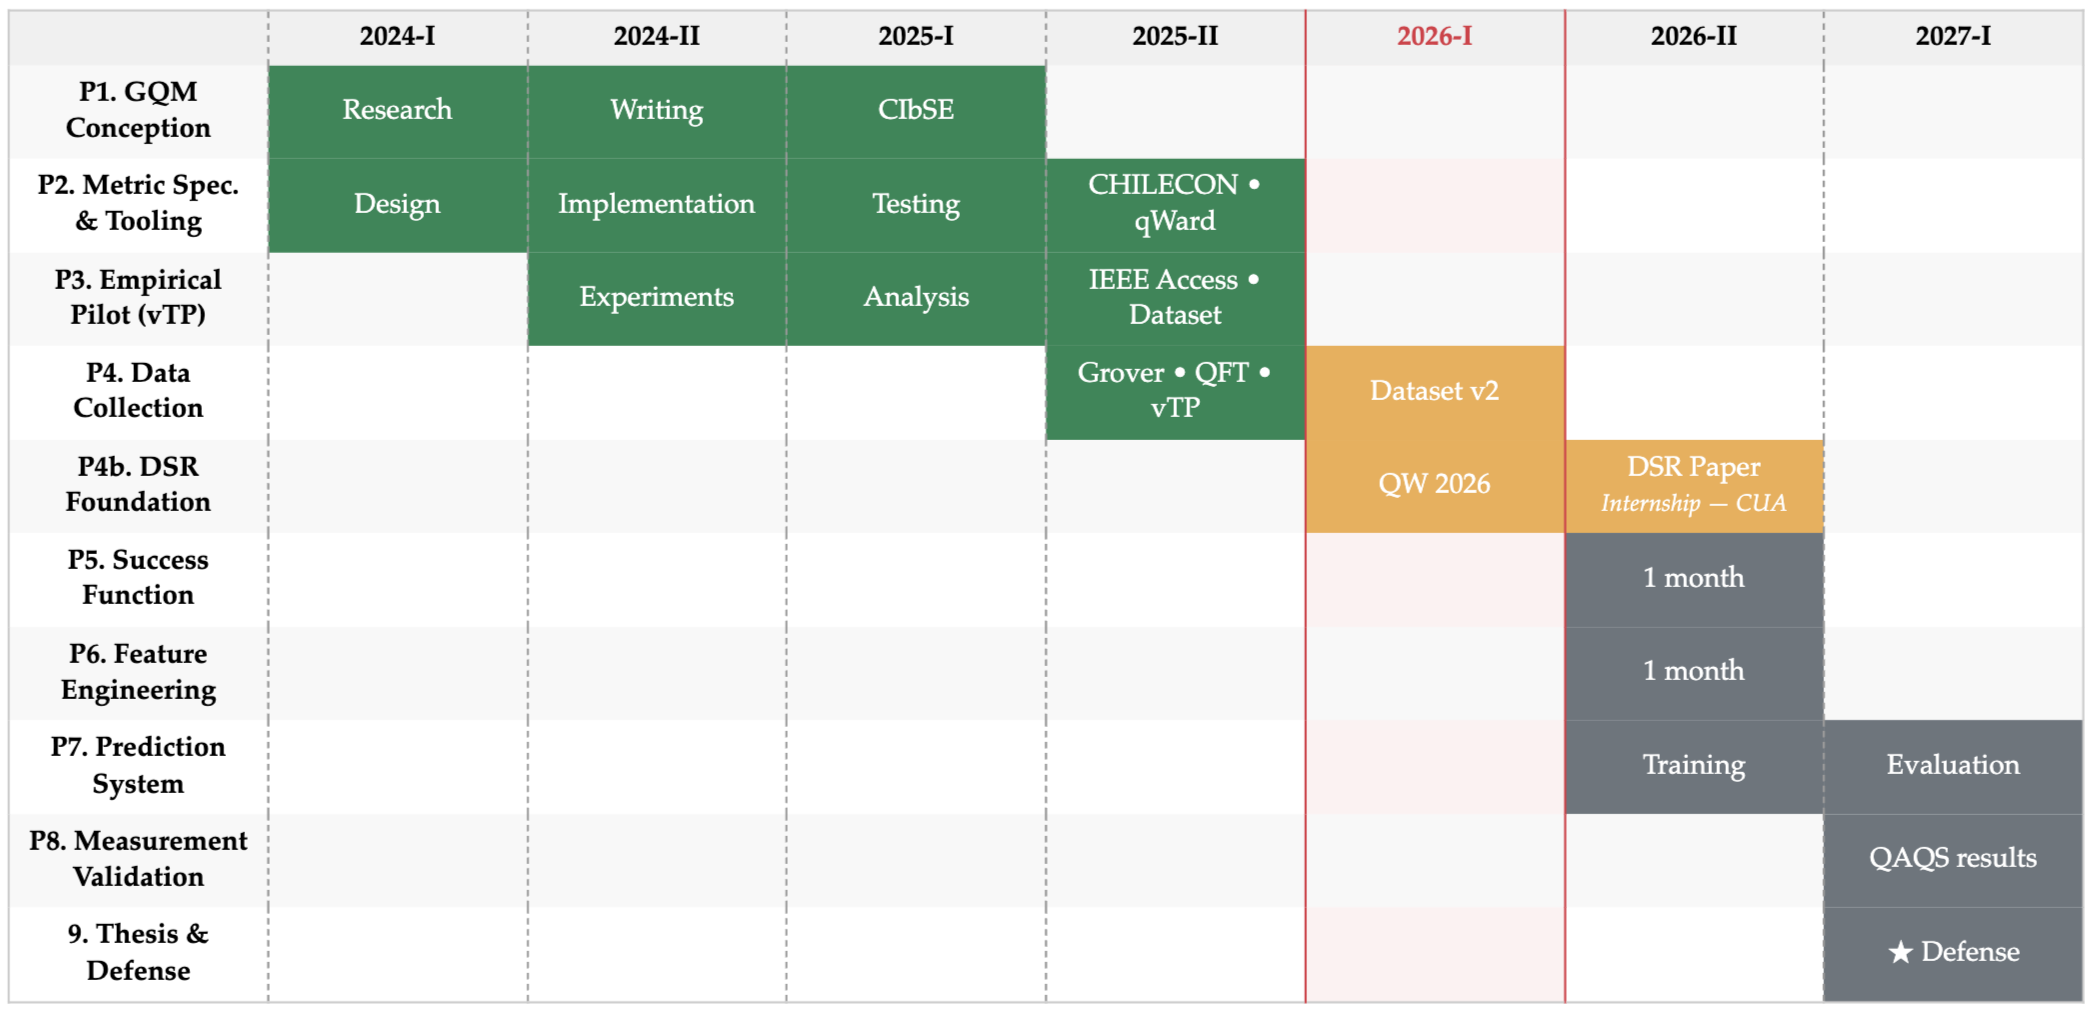
\includegraphics[width=\textwidth]{time.png}
    \caption{Visual timeline of the research phases with key publications and deliverables per semester.}
    \label{fig:timeline}
\end{figure*}

Figure~\ref{fig:timeline} complements the Gantt chart by mapping each phase to its associated publications and deliverables. Green cells denote completed work, yellow cells indicate phases that are currently in progress, and gray cells indicate proposed phases. Each publication milestone (CIbSE, CHILECON, IEEE Access, Quantum Week 2026) is placed in the semester where it was produced or submitted.

\section{AI Tools and Services Acknowledgment}

The authors acknowledge the use of AI tools and services for manuscript preparation and research assistance. Writefull.com supported language, grammar, and writing improvements; Elicit.com assisted in literature discovery; and Cursor helped with code development, including plotting scripts and quantum circuit understanding. These tools enhanced the authors' capabilities, while the core research, design, data interpretation, and conclusions are the authors' intellectual work.

\clearpage

\printbibliography

\end{document}
